%!TEX root = ../Thesis.tex

\chapter{Review of Conventional Array Imaging Approaches}

\graphicspath{{Review/Images/}}

\section{Mechanical Wave Propagation}
To understand how a wave propagates through an elastic medium, first consider a system that consists of a mass connected to a spring, as shown in Figure \ref{fig:review_massspring}. If the mass is moved from its resting state and then released, restoring forces will act upon the system until it returns to equilibrium, and these will follow the laws of harmonic oscillation. During this oscillation, potential energy in the spring is transferred to kinetic energy of the mass and vice versa. Some of this energy will be lost as it is converted to heat through friction. The mechanical properties of the mass and the spring will determine the frequency of this damped oscillation\cite{rose_basic_1979}.

\begin{figure}[ht]
\centering
		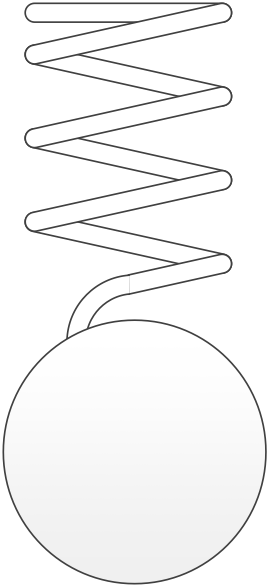
\includegraphics[width=20mm]{MassSpring3.png}
		\caption{A mass connected to a spring}
		\label{fig:review_massspring}
\end{figure}


Now consider the same system, but instead of the system being moved out of its resting state and then released, the system will be continually excited by a sinusoidally varying wave. In this case, the oscillation of the spring and the mass will match the frequency of the driving force and will maintain its amplitude while the excitation force exists.

An elastic medium can be considered as a network of `masses' (molecules) connected to each other by `springs' (elastic binding forces). If this system is excited by a sinusoidal wave, all of the `masses' in the system will oscillate with the same frequency. The `springs' will transfer the motion to each `mass' and will also introduce a delay as the kinetic energy is being transferred. This delay is known as propagation delay and is one of the fundamental and constant laws that bound wave mechanics\cite{achenbach_wave_2012}.

In an infinite solid or elastic medium, or one so large that its boundaries can be ignored, there are two kinds of stress that the medium can undergo. Therefore there are two methods of wave propagation that are possible. 

The first are longitudinal waves, named as such because the wave propagates in the same direction as the particle motion. They have the greatest wave propagation velocity in any material. The velocity of a longitudinal wave, $v_L$, can be calculated using Equations \ref{eq:review_velSolid} and \ref{eq:review_velLiquid} where $\kappa$ is Lam\'{e}'s constant, $G$ is the modulus of rigidity, $\rho$ is the material density and $\beta$ is the bulk modulus of elasticity for a fluid\cite{halmshaw_non-destructive_1991}.

\begin{equation} \label{eq:review_velSolid}
v_L = \sqrt{\frac{\kappa + 2G}{\rho}}
 \end{equation}

 \begin{equation} \label{eq:review_velLiquid}
v_L = \sqrt{\frac{\beta}{\rho}}
 \end{equation}

For a homogeneous isotropic solid with two independent material constants, the modulus of rigidity, $G$, also known as the shear modulus, can be calculated using Equation \ref{eq:review_rigid}\cite{bush_nondestructive_1989} where $E$ is the Young's modulus (the measure of the stiffness of an elastic material) and $\nu$ is Poisson's ratio (the ratio of transverse strain to longitudinal strain)\cite{boresi_advanced_1993}.

  \begin{equation} \label{eq:review_rigid}
G = \frac{E}{2(1+\nu)}
 \end{equation}

The second method of wave propagation, shear waves, propagate in a direction perpendicular to particle motion and can only exist in materials with shear elasticity (i.e. solids). The shear wave velocity, $v_S$, can be calculated using Equation \ref{eq:review_shear}. 

\begin{equation} \label{eq:review_shear}
v_S = \sqrt{\frac{G}{\rho}}
 \end{equation}

\subsection{The Wave Equation}\label{sec:wave_eq}

Wave propagation has been introduced and explained. Propagation can be  represented in a mathematical way so that it can be analysed and problems involving mechanical waves can be solved.

Consider a one-dimensional model of longitudinal waves in an elastic bar. Let the distance along the bar equal to $x$, the time equal to $t$, the cross sectional area equal to $A_{cs}$, the particle displacement equal to $u(x,t)$ and the axial force equal to $F(x,t)$\cite{morse_methods_1953}.

At any instance in time, a small element in the bar can be represented by a forces diagram, as shown in Figure \ref{fig:review_barwave}.

\begin{figure}[ht]
\centering
		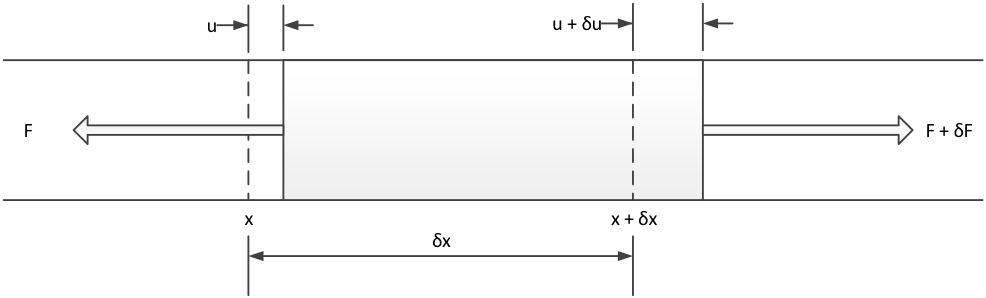
\includegraphics[width=\textwidth]{BarWave2.png}
		\caption{A `forces diagram' of a one-dimensional bar}
		\label{fig:review_barwave}
\end{figure}

From Figure \ref{fig:review_barwave}, the net force to the right can be observed. It is expressed in Equation \ref{eq:review_barwave}.

\begin{equation} \label{eq:review_barwave}
(F + \delta F) - F = \delta F
 \end{equation}

From Newton’s second law, $F=ma$, Equation \ref{eq:review_newton2} can be derived.

\begin{equation} \label{eq:review_newton2}
\delta F = \rho \frac{\delta^2 u}{\delta t^2} (A_{cs} \delta x)
 \end{equation}

Hooke's law states that the elasticity in a bar can be calculated using Equation \ref{eq:review_hooke} where $\sigma$ is stress, $E$ is Young's modulus and $\epsilon$ is strain\cite{rychlewski_hookes_1984}. 

\begin{equation} \label{eq:review_hooke}
\sigma = E \epsilon
 \end{equation}

The strain displacement relationship is given in Equation \ref{eq:review_strain}.

\begin{equation} \label{eq:review_strain}
\epsilon = \frac{\delta u}{\delta x}
 \end{equation}

Hence, Equation \ref{eq:review_strainAE} can be derived.

\begin{equation} \label{eq:review_strainAE}
F = A_{cs} \sigma = A_{cs} E \epsilon = A_{cs} E \frac{\delta u}{\delta x}
 \end{equation}

Knowing that $\delta F$ must equal $\frac{\delta F}{\delta x} \delta x$, Equation \ref{eq:review_strainAEu} can be derived from Equations \ref{eq:review_strainAE} and \ref{eq:review_newton2}.

\begin{equation} \label{eq:review_strainAEu}
\frac{\delta}{\delta x} ( A_{cs} E \frac{\delta u}{\delta x} ) \delta x = \rho \frac{\delta^2 u}{\delta t^2} (A_{cs} \delta x)
 \end{equation}

Equation \ref{eq:review_strainAEu} can be simplified into the expression shown in Equation \ref{eq:review_strainEp}.

\begin{equation} \label{eq:review_strainEp}
E \frac{\delta^2 u}{\delta x^2} = \rho \frac{\delta^2 u}{\delta t^2}
 \end{equation}

If $\frac{E}{\rho} = {v_L}^2$ and given Equation \ref{eq:review_strainEp}, the formula for a one-dimensional wave can be derived. It is represented in Equation \ref{eq:review_waveeq}.

\begin{equation} \label{eq:review_waveeq}
\frac{\delta^2 u}{\delta x^2} = \frac{1}{{v_L}^2} \frac{\delta^2 u}{\delta t^2}
 \end{equation}

The one-dimensional wave equation shows the classic feature of any wave equation: the second derivative with respect to time on one side, and the second derivative with respect to space on the other\cite{graff_wave_2012,royer_elastic_2000}.

To solve the wave equation, a displacement field must be found that satisfies the wave equation itself, as well as the appropriate boundary conditions. Analytically, it is generally impossible to solve this for both conditions, but if an infinite material is considered (i.e. a material with no boundaries), a basic solution can be found.

Equation \ref{eq:review_waveeq_sol} shows a possible solution for the wave equation, where $A$ and $B$ are unknown constants representing the amplitude of forward and backwards propagating waves respectively, $f$ is wave frequency, and $\omega$ is the angular velocity calculated by $\omega = 2\pi \cdot f$.

\begin{equation} \label{eq:review_waveeq_sol}
u(x,t) = A \cos \omega (\frac{x}{c} -t) + B \cos \omega (-\frac{x}{c} - t)
 \end{equation}

Equation \ref{eq:review_waveeq_sol} can be analysed further, given that the wavenumber can be calculated using $k = \frac{\omega}{c}$, and the solution as shown in Equation \ref{eq:review_wavenumber_sol} can be derived.

\begin{equation} \label{eq:review_wavenumber_sol}
u(x,t) = A \cos(kx - \omega t) + B \cos(-kx - \omega t)
 \end{equation}

The complex exponential equation, derived from Euler's work is shown in Equation \ref{eq:review_euler}.

\begin{equation} \label{eq:review_euler}
e^{i\theta} = \cos\theta + i \sin\theta
 \end{equation}

Only the real part of this will exist physically, and therefore Equation \ref{eq:review_wavenumber_sol} can be simplified and written as shown in Equation \ref{eq:review_wavenumber_euler}.

\begin{equation} \label{eq:review_wavenumber_euler}
u(x,t) = Re[Ae^{i(kx-\omega t)} + Be^{i(-kx-\omega t)}]
 \end{equation}

Since the subject of Equation \ref{eq:review_wavenumber_euler} is $u$, the term for displacement, the previous derivations can be used to rearrange this equation for strain.

\begin{equation} \label{eq:review_wave_strain}
\epsilon = \frac{\delta u}{\delta x} = \frac{\delta}{\delta x} Ae^{i(kx-\omega t)} = iku
 \end{equation}

Using Hooke's law, shown in Equation \ref{eq:review_hooke}, the stress-strain relationship can be written as shown in Equation \ref{eq:review_stress}.

\begin{equation} \label{eq:review_stress}
\sigma = E \epsilon = ikEu
\end{equation}

The particle velocity is the derivative of the particle displacement with respect to time.

\begin{equation} \label{eq:review_particlevel}
\dot{u} = \frac{\delta u}{\delta t} = \frac{\delta}{\delta t} Ae^{i(kx-\omega t)} = -i \omega u
 \end{equation}

The ratio between the particle velocity, $\dot{u}$ and $\sigma$ is the acoustic impedance, $Z$. Acoustic impedance is the key factor in determining energy transfer from one medium to another.

\begin{equation} \label{eq:review_acoustic_impedence}
Z = \frac{\sigma}{\dot{u}}
\end{equation}

The wave equation is linear and therefore superposition can be applied. The principle of superposition will be explored in greater depth in Section \ref{sec:huygens}. Solutions to physical problems are found by combining a number of simple solutions to satisfy the boundary conditions of the problem.

If a boundary condition is set such that the conceptual bar ends at $x=0$, the one-dimensional wave equation can be solved for this. From Equations \ref{eq:review_wavenumber_euler} and \ref{eq:review_stress} an expression can be formulated to calculate the stress at any point in the bar (Equation \ref{eq:review_solution_stress}). 

\begin{equation} \label{eq:review_solution_stress}
\sigma(x,t) = ikEAe^{i(kx-\omega t)} + ikEBe^{i(-kx-\omega t)}
 \end{equation}

The stress at $x=0$ is shown in Equation \ref{eq:review_solution_stress_x0}:

\begin{equation} \label{eq:review_solution_stress_x0}
\sigma(0,t) = ik(A - B)e^{-i \omega t}
 \end{equation}

Hence $A=B$. The final solution in terms of displacement is written in Equation \ref{eq:review_solution_displacement}\cite{feldman_derivation_2000}.

\begin{equation} \label{eq:review_solution_displacement}
u(x,t) = A(e^{i(kx-\omega t)} + e^{i(-kx-\omega t)})
 \end{equation}

If Equation \ref{eq:review_solution_displacement} is considered, it can be seen that there are two waves of equal amplitude travelling in opposite directions. One of the waves is the reflection from the end of the bar. Equation \ref{eq:review_solution_displacement} can be simplified to show that a standing wave will exist in this bar.

 \begin{equation} \label{eq:review_solution_standingwave}
u(x,t) = 2A\cos (kx)e^{-i \omega t}
 \end{equation}

If the waves in the bar are considered, a standing wave is expected if a wave is being reflected from a perfect reflector (i.e. no absorption) as the reflected wave will travel backwards exactly 180$^{\circ}$ out of phase.

\subsection{Waves at Boundaries} \label{sec:boundaries}

In ultrasonic testing, pulse echo inspection is a common method for attempting to identify flaws in materials. Reflections, and therefore echoes of incident waves, occur when a wave reaches a boundary. An ultrasonic transducer will transmit a pulse and then detect any incident waves, i.e. reflections from the transmitted signal. The signals received by the transducer can then be analysed to determine the locations of boundaries.

Consider a scenario where a longitudinal wave is travelling in a first medium towards a boundary beyond which there is a second medium. This boundary can be considered as planar and of infinite length. Equations exist to calculate the amplitude of a reflected signal given that the amplitude of the incident signal, as well as the acoustic impedance in both materials, is known.

Using the formula derived in Equation \ref{eq:review_solution_displacement}, an incident wave can be represented by the equation written in \ref{eq:review_boundaries_incident}.

\begin{equation} \label{eq:review_boundaries_incident}
u_{i} = A_{i}e^{i(k_{1}x - \omega t)}
\end{equation}

The reflected wave can be written as shown in Equation \ref{eq:review_boundaries_reflected}.

\begin{equation} \label{eq:review_boundaries_reflected}
u_{r} = A_{r}e^{i(k_{1}x - \omega t)}
\end{equation}

The wave transmitted into the second medium can be represented by Equation \ref{eq:review_boundaries_transmitted}.

\begin{equation} \label{eq:review_boundaries_transmitted}
u_{t} = A_{t}e^{i(k_{2}x - \omega t)}
\end{equation}

It must be noted the wavenumber of the transmitted wave changes, as the propagation velocity is different in the new material. For Equations \ref{eq:review_boundaries_incident} to \ref{eq:review_boundaries_transmitted}, $k_{1}$ and $k_{2}$ represent the wavenumber of the longitudinal wave in the first medium and the second medium respectively. For the boundary between the two materials, the expression shown in Equation \ref{eq:review_boundaries_amplitude} is used to relate the amplitude between each of the waves.

\begin{equation} \label{eq:review_boundaries_amplitude}
A_{i} + A_{r} = A_{t} 
\end{equation}

The pressures acting upon the boundary are also continuous and therefore Equation \ref{eq:review_boundaries_pressure} is also true.

\begin{equation} \label{eq:review_boundaries_pressure}
P_{i} - P_{r} = P_{t} 
\end{equation}

Taking Equations \ref{eq:review_boundaries_cep} and \ref{eq:review_boundaries_epc} into account, Equation \ref{eq:review_boundaries_ek} can be derived.

\begin{equation} \label{eq:review_boundaries_cep}
v_L = \sqrt{\frac{E}{P}}
\end{equation}

\begin{equation} \label{eq:review_boundaries_epc}
E = P{v_L}^2
\end{equation}

\begin{equation} \label{eq:review_boundaries_ek}
Ek = P{v_L}^2 \frac{\omega}{{v_L}} = P{v_L}\omega = Z\omega
\end{equation}

The stresses in the system can be represented by the expressions in Equations \ref{eq:review_boundaries_pressure_in} to \ref{eq:review_boundaries_pressure_trans}.

\begin{equation} \label{eq:review_boundaries_pressure_in}
P_{i} = iE_{1}k_{1}A_{i}e^{i(-\omega t)}
\end{equation}

\begin{equation} \label{eq:review_boundaries_pressure_ref}
P_{r} = iE_{1}k_{1}A_{r}e^{i(-\omega t)}
\end{equation}

\begin{equation} \label{eq:review_boundaries_pressure_trans}
P_{t} = iE_{2}k_{2}A_{t}e^{i(-\omega t)}
\end{equation}

Equation \ref{eq:review_boundaries_zA} can be derived from this.

\begin{equation} \label{eq:review_boundaries_zA}
Z_{1}A_{i} - Z_{1}A_{r} = Z_{2}A_{t} 
\end{equation}

Combining this with the previous derivations to cancel out $A_{t}$, Equation \ref{eq:review_boundaries_reflection_coefficient} can be derived, which is the definition of a reflection coefficient.

\begin{equation} \label{eq:review_boundaries_reflection_coefficient}
R = \frac{A_{r}}{A_{i}} = \frac{Z_{1} - Z_{2}}{Z_{1} + Z_{2}}
\end{equation}

Equation \ref{eq:review_boundaries_reflection_coefficient} is the proportion of the wave reflection from a boundary, which is commonly written as the reflection coefficient, $R$.

The transmission coefficient can also be calculated from this and is given in Equation \ref{eq:review_boundaries_transmission_coefficient}.

\begin{equation} \label{eq:review_boundaries_transmission_coefficient}
T = \frac{A_{t}}{A_{i}} = \frac{2Z_{1}}{Z_{1} + Z_{2}}
\end{equation}

Equation \ref{eq:review_boundaries_tr1} must be true due to conservation of energy.

\begin{equation} \label{eq:review_boundaries_tr1}
T = R + 1
\end{equation}

If a second medium is completely rigid, it will not support any particle motion. All of the energy must be reflected. $T=0$ and therefore $R$ must be equal to $-1$. If the second medium has exactly the same acoustic impedance as the first, $100\%$ of the wave will be transmitted. In this case $T=1$ and $R=0$, meaning that there will be no reflection from this interface.

If the incident wave reaches the boundary, propagating in a direction perpendicular to the boundary, then the above equations are the only ones needed to calculate what will occur. The transmitted wave will continue in a direction perpendicular to the boundary. If, however, the wave reaches the boundary at an angle, refraction will occur.

Refraction is calculated using Snell's law\cite{kuhnicke_limitations_1999}. Reflections are explained first as they the most simple interaction between a wave and an interface.

The angle of incidence is equal to the angle of reflection.

\begin{equation} \label{eq:review_boundaries_thetair}
\theta_{i} = \theta_{r}
\end{equation}

Equation \ref{eq:review_boundaries_thetair} is true for both longitudinal and shear waves. For transmission, the angle can be calculated using the expression written in Equation \ref{eq:review_boundaries_transmission_angle}. Note that $L$ stands for longitudinal, and $S$ for shear waves.

\begin{equation} \label{eq:review_boundaries_transmission_angle}
\frac{v_{L1}}{\sin\theta_{L1}} = \frac{v_{S1}}{\sin\theta_{S1}} = \frac{v_{L2}}{\sin\theta_{L2}} = \frac{v_{S2}}{\sin\theta_{S2}}
\end{equation}

Figure \ref{fig:review_snell} provides a visual representation of the refraction that occurs at a material boundary. The subscripts $_I$, $_R$ and $_T$ relate to incident, reflected and transmitted waves respectively. 

\begin{figure}[!ht]
\centering
		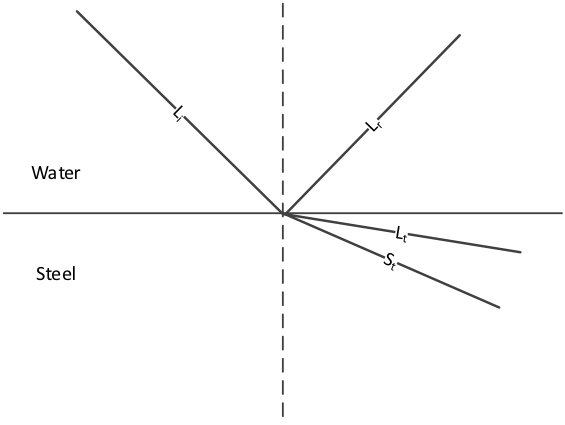
\includegraphics[width=13cm]{SnellsLaw2.png}
		\caption{An illustration of Snell's law}
		\label{fig:review_snell}
\end{figure}

When the $\theta_{2}$ reaches 90$^{\circ}$, transmission does not occur. The incident angle at which it will happen is known as the critical angle. This is important for non-destructive testing applications as if there is no longitudinal wave transmitted (and assuming that the material is a solid) only a shear wave will be transmitted. Since there is only propagation in one mode, there are many less unwanted reflections. Figure \ref{fig:review_critang1} shows what happens at the first critical angle with respect to longitudinal and shear waves; only the shear wave is transmitted.

\begin{figure}[!ht]
\centering
		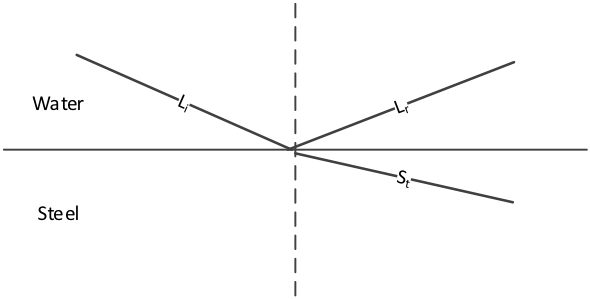
\includegraphics[width=13cm]{CritAngle12.png}
		\caption{The first critical angle}
		\label{fig:review_critang1}
\end{figure}

Equation \ref{eq:review_boundaries_transmission_angle} can be rewritten to calculate the critical angle for longitudinal waves.

\begin{equation} \label{eq:review_boundaries_crit1}
\frac{v_{L1}}{\sin \theta_{L1}} = \frac{v_{L2}}{\sin 90} 
\end{equation}

The equation can then be rearranged for $\theta_{L1}$, written in Equation \ref{eq:review_boundaries_crit1_rearranged}.

\begin{equation} \label{eq:review_boundaries_crit1_rearranged}
\theta_{L1} = \sin^{-1}\frac{v_{L1}}{v_{L2}} 
\end{equation}

To find the second critical angle, when no shear or longitudinal waves are transmitted, Equation \ref{eq:review_boundaries_transmission_angle} can be rearranged in the following way:

\begin{equation} \label{eq:review_boundaries_crit2}
\frac{v_{S2}}{\sin 90} = \frac{v_{L1}}{\sin\theta_{L1}} 
\end{equation}

\begin{equation} \label{eq:review_boundaries_crit2_rearranged}
\theta_{L1} = \sin^{-1}\frac{v_{L1}}{v_{S2}} 
\end{equation}

Figure \ref{fig:review_critang2} illustrates what happens at the second critical angle where no energy is transferred from one medium to the other.

\begin{figure}[!ht]
\centering
		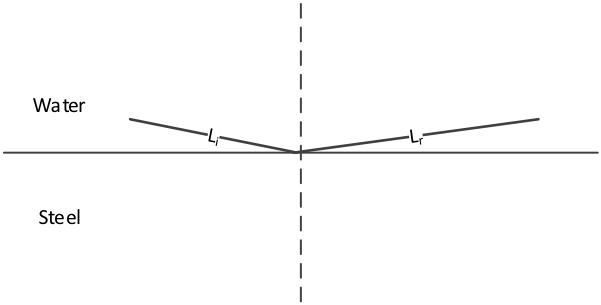
\includegraphics[width=13cm]{CritAngle22.png}
		\caption{The second critical angle}
		\label{fig:review_critang2}
\end{figure}

\section{Ultrasonic Devices}

\subsection{Ultrasound Transducers}

The definition of the word `transducer' is a device that converts one physical quantity into another\cite{transducer_concise_2006}.

An electromechanical ultrasonic transducer is an electromechanical device that converts an electrical voltage into a mechanical pressure wave or vice versa. To be classed as ultrasound the frequency of the pressure wave must be greater than the range of human hearing, which is around 20 kHz\cite{rosen_signals_2010}.

There are a number of different types of transducer, each using a different method of converting the electrical signal into mechanical motion. The most common type of transducer incorporates a piezoelectric material, which will be discussed in more detail, but there are also electrostatic, magnetostrictive and moving coil transducers. These transducers are not limited to ultrasound, but for mechanical waves in general. The moving coil transducer is similar to a commercial loudspeaker and has been used in the study of ultrasonic absorption in gases\cite{st_clair_electromagnetic_1941}. The electrostatic transducer has been used to induce ultrasonic waves in air\cite{wright_studies_1994}, but is more commonly known for driving high-end loudspeakers\cite{heydt_acoustical_2000}. Magnetostrictive transducers rely on the property of some materials where they deform when magnetised\cite{ryu_magnetoelectric_2001}.

Piezoelectric transducers are manufactured from materials that exhibit the piezoelectric effect. When a piezoelectric plate is deformed, a voltage develops between the two faces of the plate. Conversely, if a voltage is applied between two faces of a piezoelectric plate, a deformation will occur. This is known as the inverse piezoelectric effect\cite{gooberman_ultrasonics:_1969,vives_piezoelectric_2013}.

Commercial piezoelectric ultrasonic transducers are manufactured with a piezo-ceramic material at their core. Figure \ref{fig:review_transducer} shows an annotated drawing of an ultrasound transducer.

\begin{figure}[htp]
\centering
		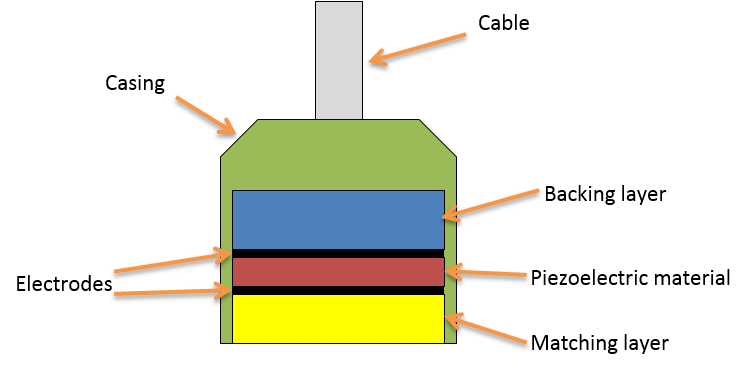
\includegraphics[width=100mm]{TransducerDiagramContrast.png}
		\caption{An annotated drawing of an ultrasound transducer}
		\label{fig:review_transducer}
\end{figure}

In Figure \ref{fig:review_transducer}, the piezoelectric material can be seen in the middle of the transducer, with electrodes on each face. Electrical wires connect the electrodes to the cable and to external instrumentation. It is the piezoelectric material that deforms when a voltage is applied between the electrodes\cite{fukumoto_design_1981}. The backing layer serves to absorb any energy that is not output from the front of the device. This is necessary to avoid excess reverberation within the piezoelectric material, which would potentially inhibit inspection due to the reverberations inducing additional voltages in the piezoelectric material. These signals would be considered coherent noise. The matching layer serves to better match the acoustic impedance of the inspection medium to the piezoelectric plate itself. This will be discussed in more depth in Section \ref{review:key_params}. The cable is required to connect the device to instrumentation, and the case protects the device as it is often mechanically sensitive. These two components also serve to shield the transducer from electrical interference. A wear layer, not depicted in the figure, is also present and protects the transducer from damages during general use. It also ensures that the device is waterproof, if appropriate for the desired application.

\subsection{Huygens' Principle}\label{sec:huygens}

A problem still to be considered is that of superposition. It has been mentioned briefly and can be used to simplify the solving of the wave equation. Superposition will now be considered in greater depth.

The wave equation is linear and this means that if $A$ and $B$ are solutions, $A+B$ is also a solution\cite{freegarde_introduction_2012}. This is the basis for many mathematical methods that consider wave fields and is can be used to explain how a group of transducers, known hereafter as an `array', can be used to manipulate a beam.

Huygens, a prominent Dutch mathematician, discovered wave superposition when he was attempting to determine, given that a wavefront is known, where subsequent wavefronts would occur. He proved his theory graphically and it was later explained mathematically by considering the known wavefront to be an infinite number of point sources\cite{baker_mathematical_2003}.

The principle of superposition can be used to calculate the wave field from a set of transducers. If a two dimensional image is considered, with length $x$ and width $z$, the pressure from a single source can be represented using Equation \ref{eq:review_huygens_pressure} where $r_j$ is the distance from the source, $P_j(x,z)$ is the pressure exerted by source, $j$, at a given point and $A_c$ is a complex number representing the amplitude and phase of the source\cite{drinkwater_ultrasonic_2006}. The $\frac{1}{\sqrt{r}}$ term is necessary for conservation of energy for a cylindrical wave coming from a line source. A line source has a similar profile to an element of an ultrasonic array. It should be noted that this equation is an approximation and is not valid in the near field (calculated by $\frac{D^2}{4\lambda}$ where D is the source width) due to the rapid fluctuations of amplitude that occur in this region. 

\begin{equation} \label{eq:review_huygens_pressure}
P_j(x,z) = A_c \frac{1}{\sqrt{r_j}} e^{i(kr_j - \omega t)}
\end{equation}

This can be summed for all point sources to get the total wave field with all sources considered. In Equation \ref{eq:review_huygens_wavefield}, $n$ is the number of sources in the system. 

\begin{equation} \label{eq:review_huygens_wavefield}
P(x,z) = \sum_{j=1}^{n} A_c \frac{1}{\sqrt{r_j}} e^{i(kr_j - \omega t)}
\end{equation}

For an array of point sources, Equation \ref{eq:review_huygens_wavefield} can be written as an integral, where $r'$ is the distance from the point $(x,z)$ to the point on the array, that is distance $x'$ from the centre. $a$ is the width of the transducer.

\begin{equation} \label{eq:review_huygens_wavefield_integral}
P(x,z) = \int_{-\frac{a}{2}}^{\frac{a}{2}} A_c \frac{1}{\sqrt{r'}} e^{i(kr' - \omega t)} dx'
\end{equation}

Equation \ref{eq:review_huygens_wavefield_integral} can often be solved by adopting assumptions, making the solution only valid in the far field, but greatly simplifying it to the point where it can be solved analytically. Equations \ref{eq:review_huygens_wavefield_polar} to \ref{eq:review_huygens_wavefield_solved} show a solution for the field of a transducer, valid only for the far field.

The integral in Equation \ref{eq:review_huygens_wavefield_integral} can be expressed in terms of polar co-ordinates where $r' = \sqrt{R^2 + x'^2 - 2Rx'\cos(90 - \phi)}$. $R$ is the distance from the array centre and $\phi$ is the angle of the array centre with respect to the normal.

\begin{equation} \label{eq:review_huygens_wavefield_polar}
P(R,\phi) = \int_{-\frac{a}{2}}^{\frac{a}{2}} \frac{1}{\sqrt{r'}} e^{i(kr' - \omega t)} dx'
\end{equation}

It is also assumed that $P$ is in the far field and it is assumed that $R$ is much greater than $x'$ and so, due to these assumptions, the following is true.

\begin{equation} \label{eq:review_huygens_assumption1}
r' \approx R - x'\sin\phi
\end{equation}

\begin{equation} \label{eq:review_huygens_assumption2}
\frac{1}{\sqrt{r'}} \approx \frac{1}{\sqrt{R}} 
\end{equation}

The integral can then be rewritten taking these assumptions into account.

\begin{equation} \label{eq:review_huygens_wavefield_phi1}
P(R,\phi) \approx \int_{-\frac{a}{2}}^{\frac{a}{2}} \frac{1}{\sqrt{R}} e^{i(k(R - x'\sin\phi) - \omega t)} dx'
\end{equation}

\begin{equation} \label{eq:review_huygens_wavefield_phi2}
P(R,\phi) \approx \frac{1}{\sqrt{R}} e^{i(kR - \omega t)} \int_{-\frac{a}{2}}^{\frac{a}{2}} e^{i kx' \sin\phi} dx'
\end{equation}

If Equation \ref{eq:review_huygens_wavefield_phi2} is integrated, the final equation for the field from a signal rectangular element in the far field is derived.

\begin{equation} \label{eq:review_huygens_wavefield_solved}
P(R,\phi) \approx \frac{a}{\sqrt{R}} e^{i(kR - \omega t)} \frac{sin(\frac{1}{2} ka \sin\phi)}{\frac{1}{2} ka \sin\phi}
\end{equation}

Huygens' principle has shown that a line source can be integrated across and a solution derived for the pressure field of this transducer. An array of ultrasonic transducers can be considered as a group of sources and thus the pressure field from an array can be calculated using the above methodology. The field from each element in the array can be determined individually and then summed to find the field for the full array. 

The directivity function defines how the pressure in a field varies with the angle from the transducer. The directivity of an element is a function of the width of the element and the wavelength of the emitted wave.

\begin{equation} \label{eq:review_huygens_directivity}
D_F(\phi) = \frac{\sin(\frac{1}{2} ka \sin\phi)}{\frac{1}{2} ka \sin\phi} = \textrm{sinc}( \frac{1}{2} ka \sin\phi ) = \textrm{sinc}(\frac{\pi a \sin \phi}{\lambda})
\end{equation}

The delay required from each element in a transducer array required to achieve focus at any point in the far field of the image can be calculated. The centre element is chosen to have a delay of $0$ and the relative time delays for each other element can be calculated.

\begin{equation} \label{eq:review_huygens_delay}
t_j = \frac{d_j - d_0}{v}
\end{equation}

Equation \ref{eq:review_huygens_delay} shows a simple equation to calculate each element's time delay, where $v$ is the velocity in the medium, $d_j$ is the distance to element $j$ from the focal point, and $d_0$ is the distance to the reference element (the centre element, in this case). This is then converted to a phase delay, $B_j$, so that the term can be used in the frequency domain and applied as a transfer function.

\begin{equation} \label{eq:review_huygens_delay_phase}
B_j = e^{i\omega t_j}
\end{equation}

With this knowledge, an equation can be written to calculate the wave field in the far field from an array element, complete with beam focusing and directivity.

\begin{equation} \label{eq:review_huygens_wavefield_final}
P(x,z) = \sum_{j=1}^{n} B_j D_f(\phi_j) \frac{1}{\sqrt{r_j}} e^{i(kr_j - \omega t)}
\end{equation}

Figure \ref{fig:review_huygens} shows the wave field of a 32 element array employing beam steering. This pressure field was computed using a software implementation of Equations \ref{eq:review_huygens_directivity} to \ref{eq:review_huygens_wavefield_final}. Note that the pressure field from the beam is off-centre due to the beam steering, and also the complexity of the field within the `near-field' which shows graphically why simple assumptions cannot be made for modelling the near-field.

\begin{figure}[ht]
\centering
		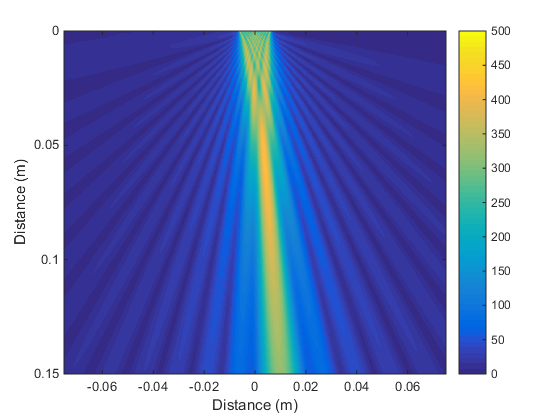
\includegraphics[width=10cm]{WaveField3.png}
		\caption{A wave field, calculated programmatically using an implementation of the theory in this section. Shown with a linear scale.}
		\label{fig:review_huygens}
\end{figure}

\subsection{Ultrasound Arrays}

An ultrasonic array can be simply defined as an arrangement of two or more ultrasonic transducers\cite{thurstone_ultrasonic_1965}. Each transducer is referred to as an element of the array. Each element in the array can be driven independently of, or along with, any other element. This allows for phased array ultrasonic testing. Arrays are available in either 1D, 2D or annular configurations. Figures \ref{fig:1D_array} to \ref{fig:annular_array} show examples of element layouts for each configuration. Additionally, a photograph of a 2D commercial array (Imasonic, France) is shown in Figure \ref{fig:review_arraypic}.

\begin{figure}[htp]
\centering
		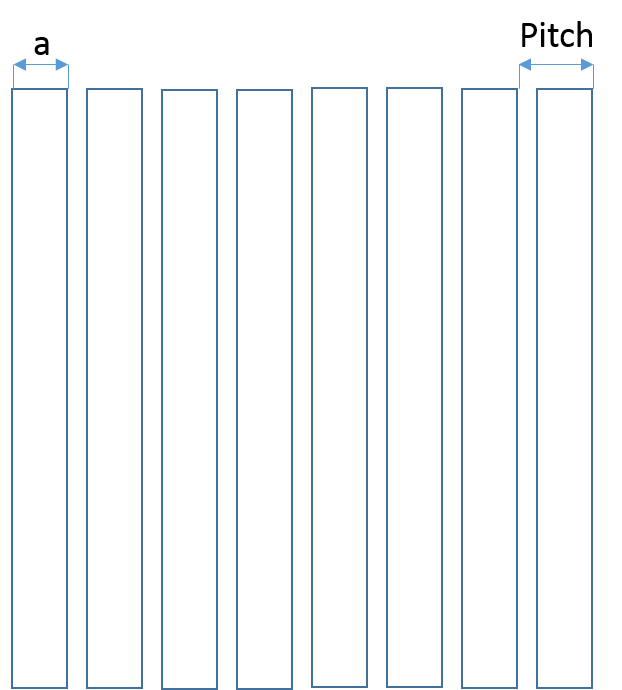
\includegraphics[width=70mm]{Array_1D.png}
		\caption{An example element layout for a 1D array}
		\label{fig:1D_array}
\end{figure}

\begin{figure}[htp]
\centering
		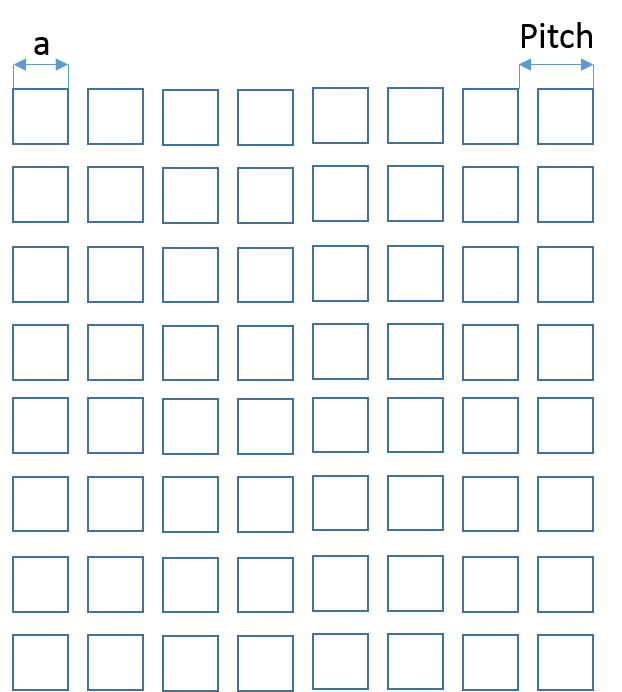
\includegraphics[width=70mm]{Array_2D.png}
		\caption{An example element layout for a 2D array}
		\label{fig:2D_array}
\end{figure}

\begin{figure}[htp]
\centering
		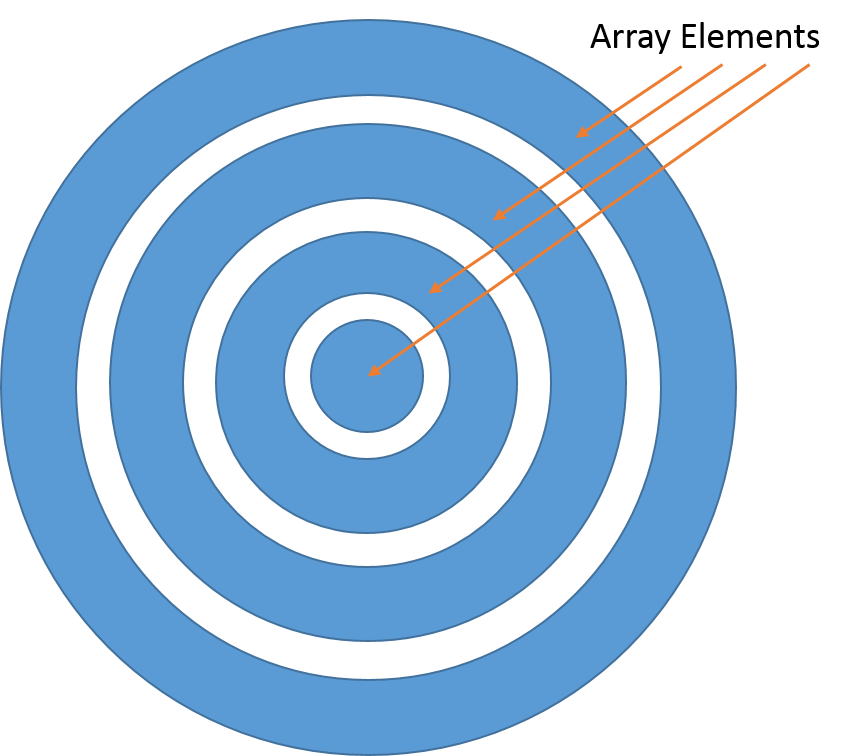
\includegraphics[width=70mm]{Array_annular.png}
		\caption{An example element layout for an annular array}
		\label{fig:annular_array}
\end{figure}

\begin{figure}[htp]
\centering
		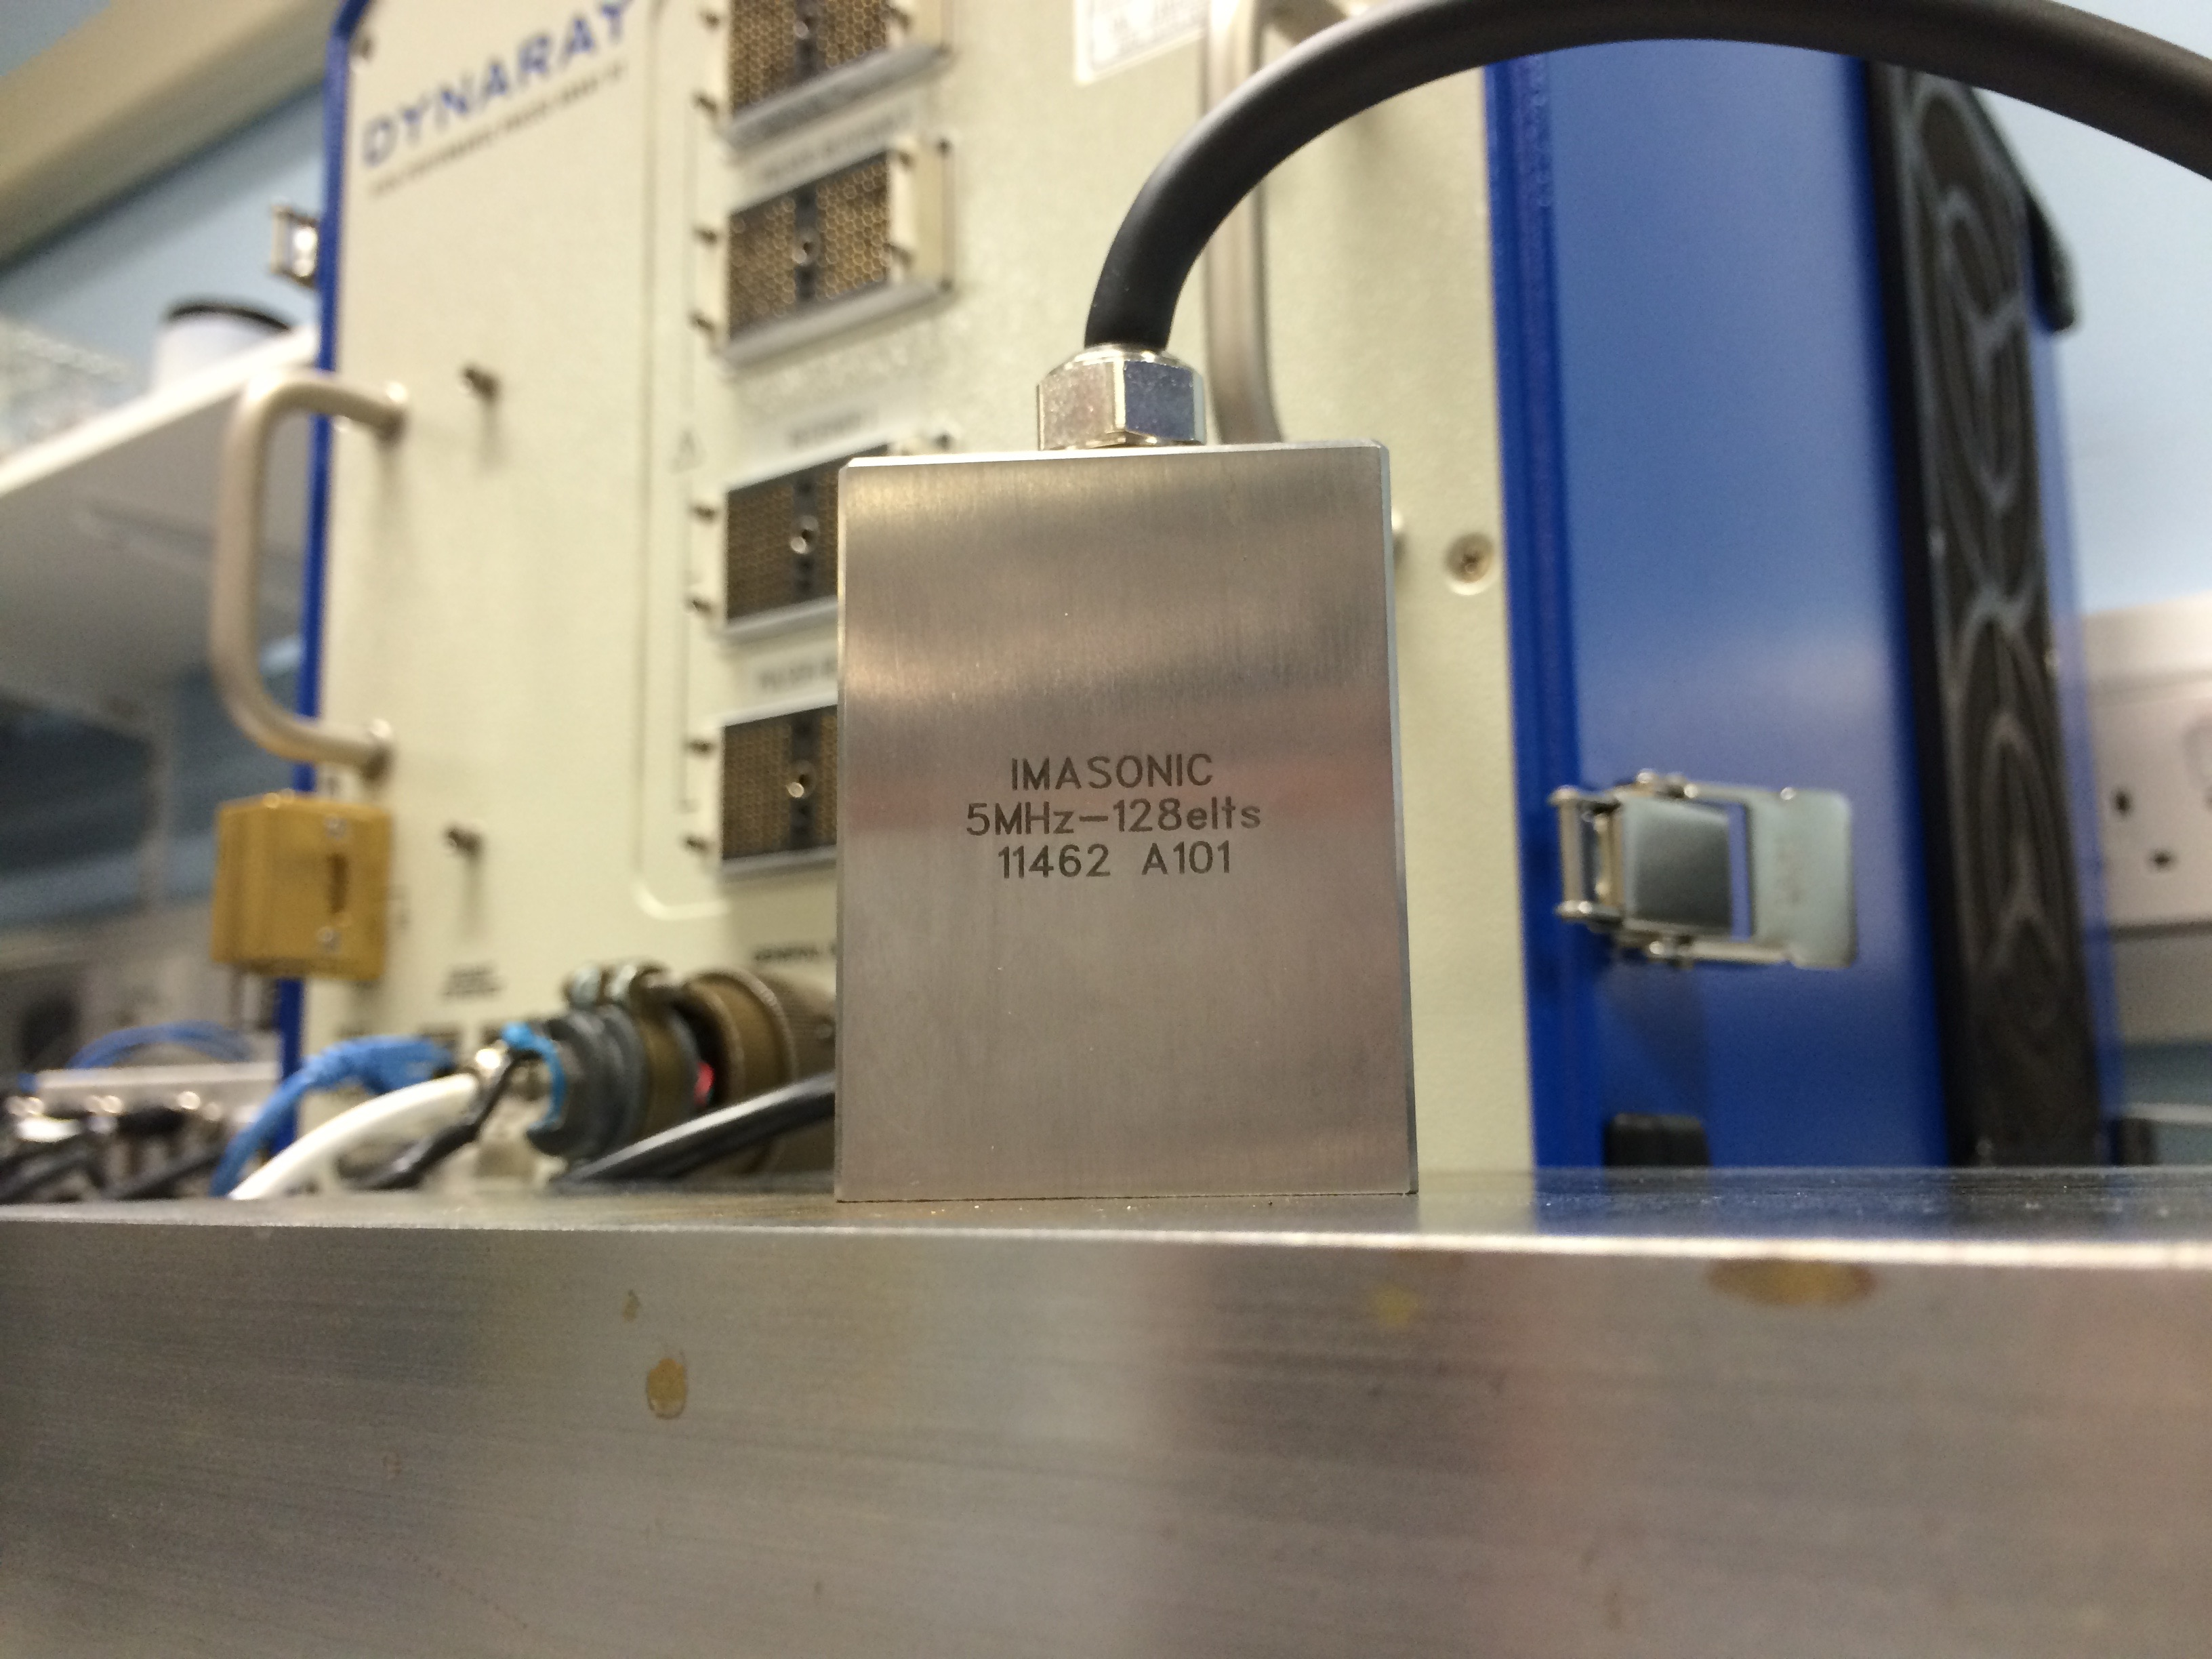
\includegraphics[width=100mm]{Array.jpg}
		\caption{A commercial two-dimensonal array}
		\label{fig:review_arraypic}
\end{figure}

In this thesis, a commercial linear array (Vermon, France) was used for all experimentation. The parameters of this probe are shown in Table \ref{table:vermon_5mhz}.

\begin{table}[htbp!]
\begin{center}
	\begin{tabular}{| c | c |}
	\hline 
	\textbf{Parameter} & \textbf{Value} \\ \hline \hline 
	Centre Frequency	& 5 MHz \\ \hline
	Element Count & 128 \\ \hline
	Pitch & 0.7 mm \\ \hline
	Layout & Linear \\ \hline
	\end{tabular}
	\caption{Vermon array parameters for step wedge inspection}
	\label{table:vermon_5mhz}
	\end{center}
	\end{table}


\subsection{Ultrasound Arrays Versus Single Element Probes}

Single element probes exert a pressure load onto the inspection medium, creating a mechanical wave that will disperse in the medium. The probe will pick up any received waves and convert them to electrical energy which can then be manipulated for observation. Due to the wave propagating spherically, reflectors do not necessarily have to be directly under the probe\cite{alleyne_optimization_1992}. This makes it difficult to locate a defect within a medium if there are a number of off-axis reflectors\cite{lazaro_influence_2002}. This can be partly solved by using a directional probe. In this case the surface of the probe is slightly concave and will have a depth at which all the emitted energy is focused at one point\cite{thurstone_ultrasonic_1965}. The energy from off-axis signals is reduced and one can be more certain that any reflections are within the expected wave path of the probe\cite{buddemeyer_physics_1975}. With each of these methods the standard way to interpret this data is to view or process the one dimensional amplitude signal in the time domain, also known as an A-scan\cite{santodomingo-rubido_new_2002}.

The benefit of using an array for these problems is that the focus is not fixed and can be changed on the fly, during an inspection. The wavefront can be dynamically steered, focused, or both. Furthermore, the use of Full Matrix Capture allows a user to generate datasets and apply signal processing techniques in post-processing. The use of phased array also allows for beam steering, meaning a larger area can be inspected in the same amount of time when compared to single element inspection.

There are few downsides to using an array over a single element probe. The first is cost. To exploit ultrasonic arrays to their full potential, a Phased Array Controller (PAC) is required. These range in cost from thousands of pounds to hundreds of thousands of pounds. The connectors for these arrays are also expensive. While almost all single element probes use standard co-axial connectors, commercial arrays will use one of a number of proprietary connectors.

Most PACs are bundled with the manufacturer's software which is used to drive the array. It is often difficult to export the data from this software into a file that can be opened by other programs. This is in contrast to a single element probe that can be operated with a simple signal generator and an oscilloscope.

The final drawback of arrays is the typical element size. Arrays need to be of a size and weight such that operators can use them comfortably. It means that a large number of elements are required to fit in a comparatively small space, leading to a small element size. The narrow spacing is also necessary to avoid grating lobes which occur when the element spacing is greater than half the wavelength in a periodic array. This has a direct effect on how much energy each element can impart to the inspection medium, as well as the sensitivity of the element.

\subsection{Key Array Parameters for Design and Inspection}\label{review:key_params}

Similar to single element inspection, an appropriate ultrasonic array must be selected for a given inspection. Some parameters are more important than others depending on the type of inspection.

The majority of commercial arrays for NDE are either linear (one-dimensional) or matrix (two-dimensional), and are periodic, meaning that the element spacing is the same for each element. 1D arrays have larger element sizes leading to an increased sensitivity and it is generally simpler to create focal laws for these devices. 2D arrays often offer a complex arrangement of elements and can used for volumetric imaging. Annular arrays are used when a variable focus is required, and can be used in place of single element transducers that are focused using hardware\cite{drinkwater_ultrasonic_2006}.

`Sparse' layouts are also available, where the elements are more spread out than a standard probe and may not be spaced linearly. Care must be taken when choosing a sparse array as if an regular, periodic array has an element spacing greater than $\frac{\lambda}{2}$ (where $\lambda$ is the wavelength) grating lobes will be present\cite{harrington_sidelobe_1961}. Energy distribution patterns, or lobes, will be discussed in greater detail in Section \ref{sec:lobes}. 2D arrays allow for a complex layout of elements such as the one shown in Figure \ref{fig:review_sparse_array}, which is the element layout of the array shown in the photograph in Figure \ref{fig:review_arraypic}. These complex array layouts can allow for a greater sensitivity over a larger area. The amplitude of sidelobes can often be reduced in post-processing\cite{seo_sidelobe_2008}.


\begin{figure}[htp]
\centering
		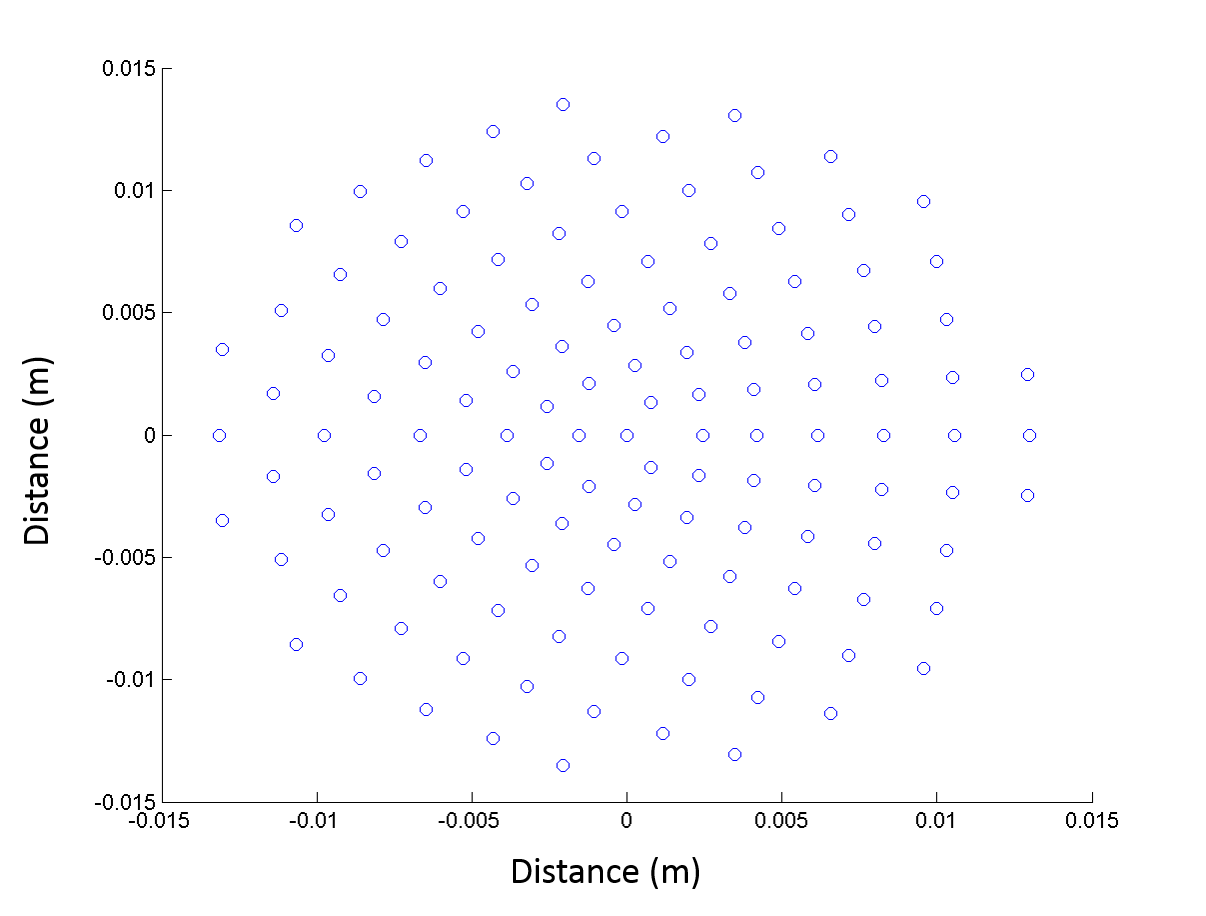
\includegraphics[width=100mm]{SparseArrayLocations_axes.png}
		\caption{An example of element locations on a 128 element sparse array}
		\label{fig:review_sparse_array}
\end{figure}


The array must also be properly matched to the inspection medium. As with high frequency electromagnetic signals transmitted along a wire, a significant impedance mismatch between two media can result in the majority of the energy being reflected at the boundary and little transfer of energy into the sample itself. This can be approached in two ways. Arrays generally have a matching layer, which is an intermediate step between the acoustic impedance of the device and of the target material. In order to ensure an efficient transfer of energy, matching layers are often complex and include multiple layers of materials. Wedges, which can be used to steer a beam, can also be used as a tool for matching. It is common for commercial arrays to be matched to Rexolite\cite{rexolite_web} or other such wedge materials.

The centre frequency of a probe is a key parameter in determining the performance of an ultrasonic testing system. High frequency waves are attenuated to a greater extent and interact with much smaller particles within a medium of inspection when compared to waves of a lower frequency. Difficult materials often have grains that are of a size that interferes with the propagation of high frequency ultrasonic signals. The wavelength of the wave determines the size of particles that will interact with the wave. Generally, grains or particles with a size greater than half-wavelength ($\frac{\lambda}{2}$) will interact with incident waves. This interaction is desirable when attempting to locate small defects. The drawback of using a lower frequency probe is twofold. Lower frequencies lead to a lower spatial resolution as small features will not be resolved\cite{simonetti_multiple_2006}. Lower frequency probes take a longer time to reach an equilibrium after an excitation. The time taken to reach this equilibrium after the initial excitation is known as the ringdown time. While the transducer is returning to a steady state after the excitation, any energy received will not appear as a significant contribution to the energy within the probe. Hence, a long ringdown time means that areas close to the transducer cannot be inspected using conventional methods. Figure \ref{fig:review_ringdown} shows an A-scan of a low frequency probe emitting a signal into a Rexolite sample. The long ringdown time of this probe can be clearly observed in the first 20${\mu}s$ of this image, where saturation can also be observed. Problems with long ringdown times can be overcome using a stand-off, but unless the stand-off has the same acoustic impedance and ultrasound propagation velocity as the sample, reflections will occur and refractions will add complexity to the focal law generation.

\begin{figure}[htp]
\centering
		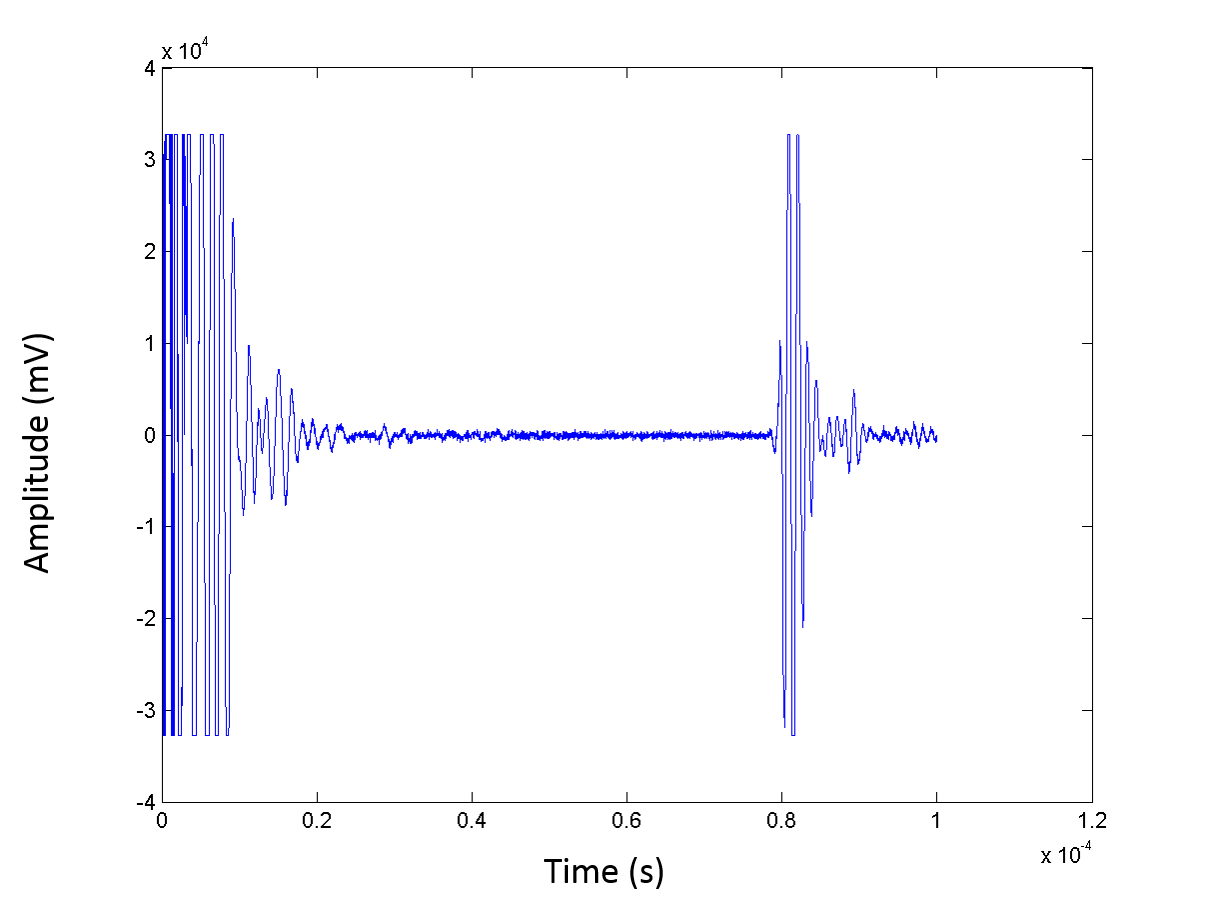
\includegraphics[width=100mm]{Ringdown_axes.png}
		\caption{The response of an element from interrogating a Rexolite block with 1 MHz linear array}
		\label{fig:review_ringdown}
\end{figure}

All ultrasonic transducers have a finite frequency response giving rise to an effective bandwidth. The bandwidth is measured relative to its maximum amplitude response in the frequency domain and a transducer is considered responsive until the magnitude of the response falls below half of the maximum value. A typical frequency response curve for a commercial array is shown in Figure \ref{fig:review_freqresponse}. Bandwidth can be measured in Hertz or as a fraction of the centre frequency of the array. Commercial probes have a fractional bandwidth ranging between 30\% to over 100\%\cite{nowicki_influence_2007}. Bandwidth becomes important for advanced post-processing where the frequency domain signal is manipulated in order to remove noise and other unwanted signals. A higher bandwidth probe means that there is more frequency content to work with. It also means that the signal can be more truly reconstructed.

\begin{figure}[htp]
\centering
		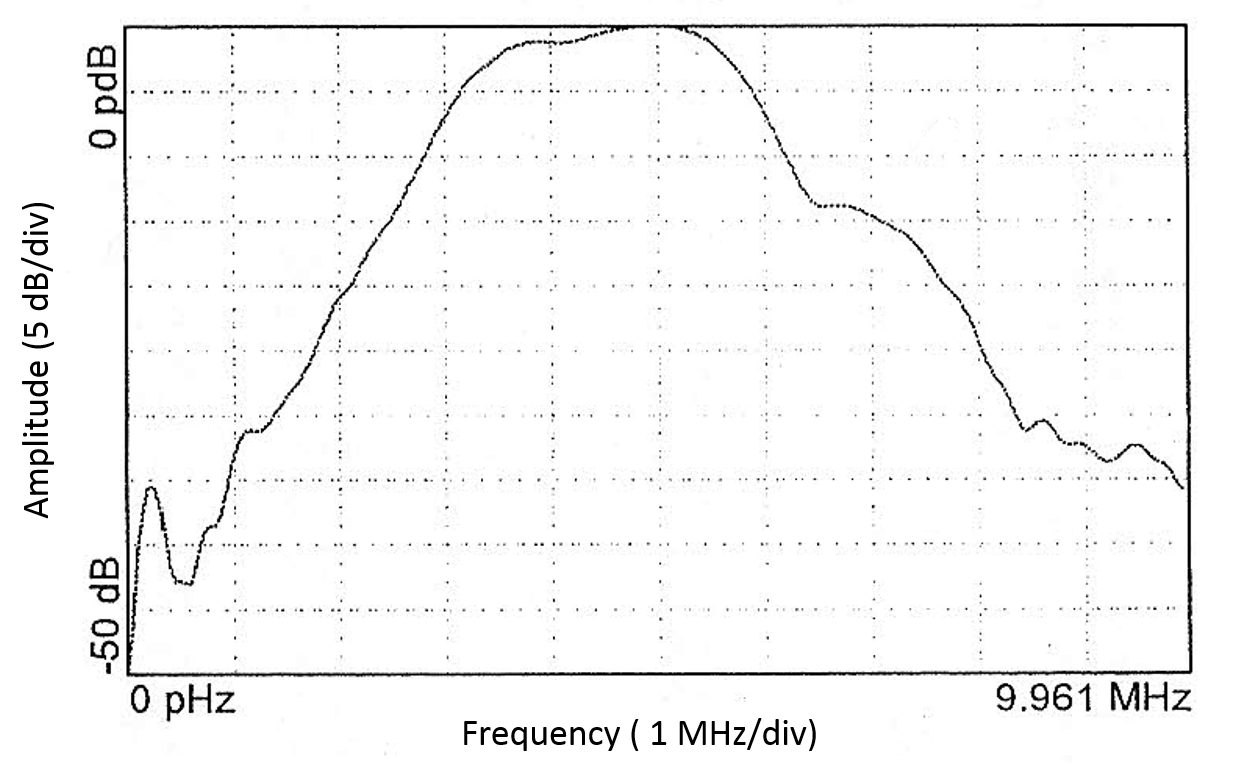
\includegraphics[width=100mm]{FreqResponse_axes.png}
		\caption{The frequency response for a commercial 5 MHz linear array, scanned from a datasheet (Vermon, France).}
		\label{fig:review_freqresponse}
\end{figure}

It is often difficult to find an off-the-shelf commercial probe for specialised applications, however a number of array manufacturers will manufacture custom probes to a customer's specification. In these cases, the customer is expected to provide the desired element locations, centre frequency and required bandwidth. Arrays that have a high fractional bandwidth (\textgreater 100\%) are well suited to acquisition for the purpose of frequency-domain specific post-processing.

The surface geometry of elements is often not square. The Vermon 5MHz linear 128 element 1D array used in this thesis has elements with a pitch of 0.7mm, length of 0.5mm in the direction of the primary axis and width of 10mm in the direction of the secondary axis. This rectangular shape makes the elements directional. This property is beneficial for a one dimensional array as one does not want to receive off-axis signals. The physical properties of each element also reduce the sensitivity to signals arriving from extreme angles. The angular sensitivity for an array element primarily depends on its width and the operating frequency. 

\section{Array Imaging}

There are many ways to create an image from data acquired from an ultrasonic array. This section will deal with the concept of beamforming and introduce array imaging to support understanding of advanced array processing discussed in subsequent chapters. 

Fermat stated that the path a ray of light takes between two points is the path that can be traversed in the least amount of time\cite{schuster_introduction_1904} (it is this that gives rise to Snell's law, introduced in Section \ref{sec:boundaries}). This principle also holds true for ultrasound\cite{connolly_application_2009}. 

Instead of considering ultrasound energy as a moving wavefront, it can instead be thought of as a ray. This simplifies many imaging algorithms.

It must be noted that while images can be created more easily when taking this principle into account, the wavefront still exists and will contribute to noise if there are any off-axis reflectors. The algorithms in this section will treat the ultrasonic wave as a wavefront if more than one element is being excited at any time, and a ray if only one element is being excited at a time.

The most simple way to display ultrasonic data is via an amplitude scan (A-Scan). It is a plot of amplitude against time for a single ultrasonic receiver. A typical A-Scan is shown and annotated in Figure \ref{fig:review_ascan}.

\begin{figure}[htbp]
\centering
		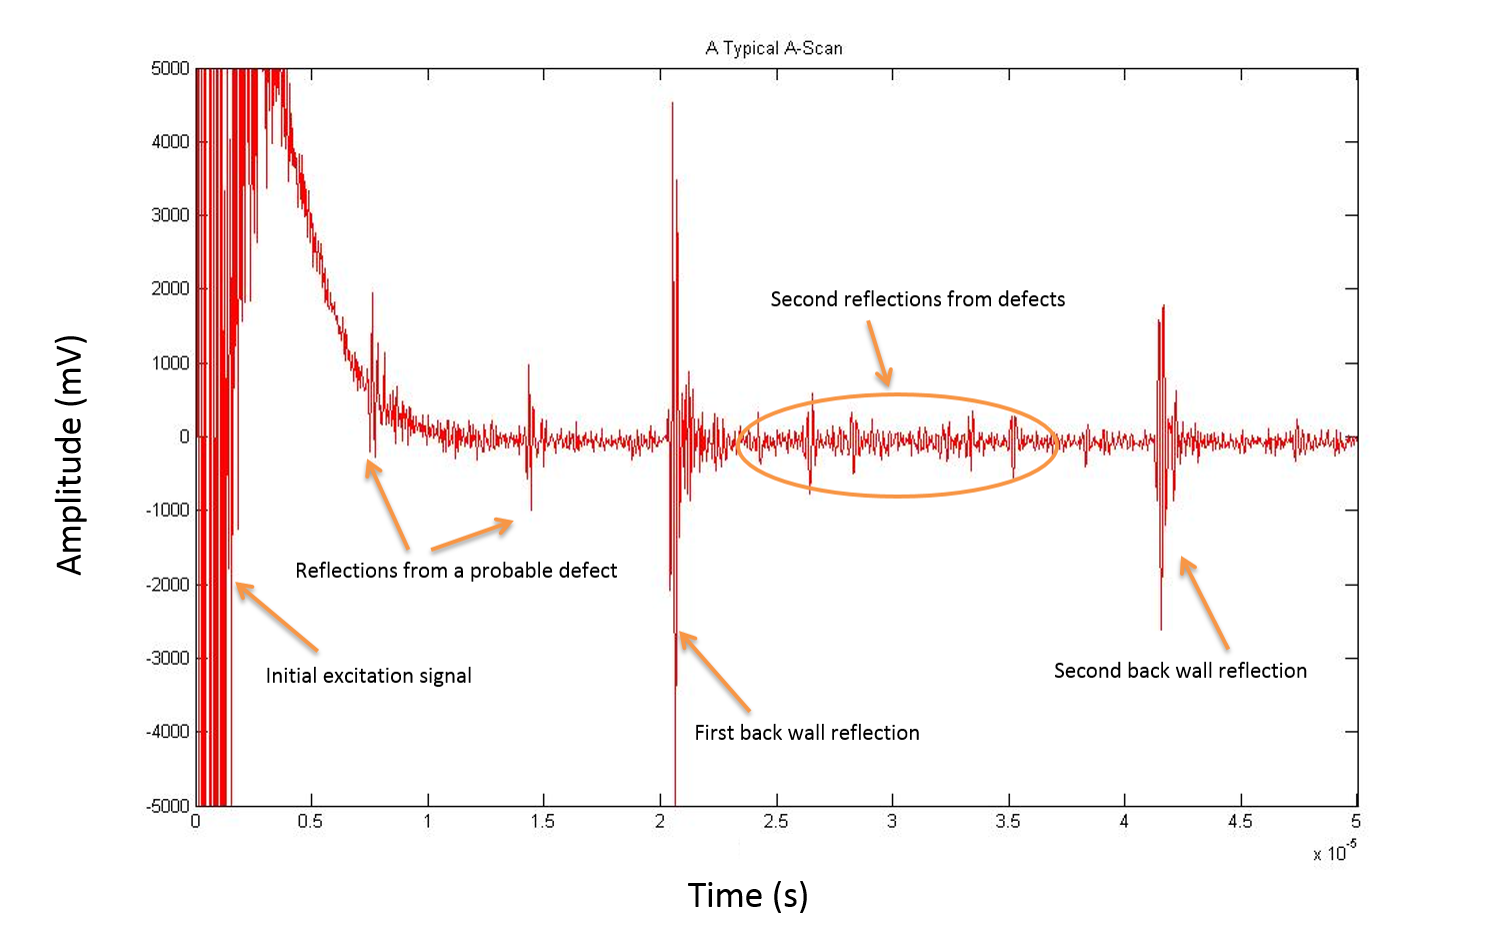
\includegraphics[width=\textwidth]{AScan2_axes.png}
		\caption{An annotated A-Scan}
		\label{fig:review_ascan}
\end{figure}

The A-Scan in Figure \ref{fig:review_ascan} shows an initial excitation, two reflections from features within the medium and a larger reflection from the back wall of the medium. The second reflection from the back wall is also visible.

A-Scans are useful for detecting the presence of a reflector in a material which is ultrasonically clean (that is, one which does not have large grains). The depth of a reflector can be calculated, given the knowledge of the wave propagation velocity and the time where the reflection occurred. 

More information about a defect can be gained through the use of arrays. Arrays allow a larger volume to be inspected from a single position and also allow for defect sizing and characterisation. They also allow for representing data using B and C scans.

The quality of images is often quantitatively measured using a metric known as Signal to Noise Ratio (SNR). SNR is a ratio of the amplitude of the desired signal to the amplitude of the background noise and is commonly represented in decibels (dB).

\subsection{Phased Array Imaging}\label{sec:lobes}

Phased array imaging at its most basic is the use a phased array controller to excite a number of elements in an array with a set of delay laws intended to focus or steer the beam. The data received by each element is then processed and combined in order to create an A-scan. When the transmitted signal from more than one element is summed to generate a focused wavefront, a set of lobes are formed\cite{smith_High-speed_1991}. Figure \ref{fig:review_lobes} shows a typical lobe pattern from an array. This image was generated by Kummer et al\cite{kummer_ultra-low_1963}. The largest lobe, travelling in the primary steering direction, is known as the main lobe. Side lobes are also generated as an additional effect of generating the interference pattern. These are attached to the main lobe but radiate energy in undesired directions. These often contribute to noise by causing off-axis reflections. Grating lobes are outputs of focused energy created when the element spacing is over $\frac{\lambda}{2}$. These can also contribute to noise. The choice of element layout can help to reduce the amplitude of these undesirable lobes\cite{harrington_sidelobe_1961}.

\begin{figure}[htbp]
\centering
		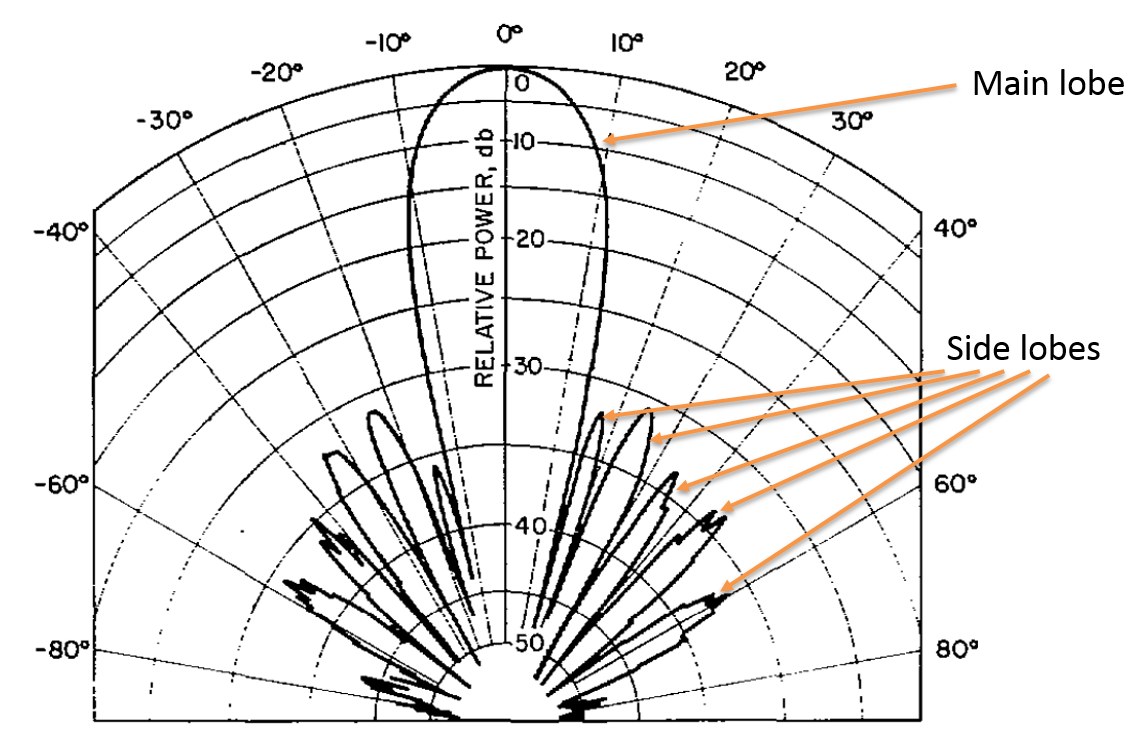
\includegraphics[width=100mm]{Lobes2.png}
		\caption{A typical lobe pattern generated from an array}
		\label{fig:review_lobes}
\end{figure}

\subsubsection{The Focused B-Scan}

By applying delays on transmission, ultrasonic energy can be focused at a single point. This will increase the amplitude of reflections from this point, increasing the signal-to-noise ratio\cite{long_ultrasonic_2012} (SNR). By applying these same delays at the time when the data is received, the transmission delays can be accounted for, and the contribution from each element summed to create a A-Scan where the energy is focused.

Figure \ref{fig:FocusedB} illustrates how a focused B-scan is applied to inspect a range of locations using phased array. A sub-aperture of the array is used to generate a focused wavefront which can be moved by shifting the delay laws to different elements along the entire aperture of the array.

\begin{figure}[htbp]
\centering
		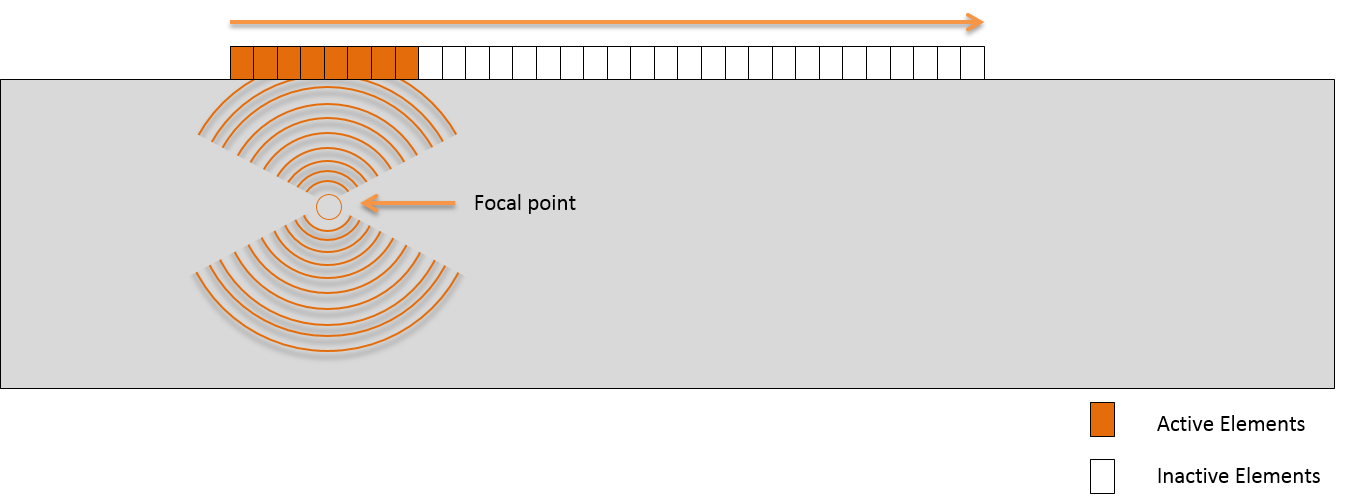
\includegraphics[width=\textwidth]{FocusedB.png}
		\caption{An illustration of the focused B-scan}
		\label{fig:FocusedB}
\end{figure}

To focus at a single point a frame of reference must first be established, from which all delays are calculated with respect to the reference point. This is usually chosen to be the centre of the sub-aperture. The time taken for a wave to propagate from the centre of the array to the point at which the beam will focus is calculated using Equation \ref{eq:review_bscan_prop_time}, where $x$ is the the distance of the focal point parallel to the array, $z$ is the distance to the focal point perpendicular to the array, and $v_L$ is the longitudinal propagation velocity. The point can be off-axis, relative to the array, but is limited by the directionality of the array elements.

\begin{equation} \label{eq:review_bscan_prop_time}
T = \frac{\sqrt{ x^2 + z^2 }}{v_L}
\end{equation}


For every element on the array other than the centre one, the time taken for a wave to propagate to the focal point is calculated and subtracted from the time calculated in Equation \ref{eq:review_bscan_prop_time}. This gives the delay to be applied to each element. A negative delay indicates that the pulse should lead the reference time (i.e. should be excited before the reference $t=0$).

On reception, the opposite delays can be applied to that the received A-scans may be summed together and plotted. This style of processing can be referred to as delay-and-sum. It is the basis of all of the other focused B-Scan techniques discussed in this section.


\subsubsection{Dynamic Depth Focusing}

The classic delay-and-sum methodology will result in a processed A-scan which is focused at the point of interest. All other points will be defocused. 

It is possible to amend the delays applied on receiving in order to focus at multiple depths in a medium\cite{chatillon_simulation_2009}. This is called dynamic depth focusing (DDF) and is an example of the kind of post-processing available on ultrasonic arrays. With a single transmission with fixed focus, variable focal laws on receive allow the modification of focus through a range of points.

DDF quantises the path the beam travels into a number of focal zones. These zones can be infinitely divided, allowing for a different focal law for each sample in the processed A-scan, or can cover a large area to limit the number of focal laws. The latter can be useful when implementing DDF into hardware where memory and processing time is a concern.

For a focal zone, the focal point is defined as the centre of the zone. From there, the receive portion standard delay-and-sum algorithm is applied. This is repeated for every focal zone defined along the beam's path. In this case, the only true focus is where the beam is focused at the time of transmission but the pseudo-focusing performed in DDF makes the a larger portion of the A-scan in focus, as opposed to only a small range of samples.

\subsubsection{Sector Scanning}

After DDF has been applied, the result will be a well focused A-scan valid for the beam path from the point of reference on the array, to beyond the initial point of focus.

This can be repeated across an arc to create a sweep of focal points throughout a slice of a volume. Combined with dynamic depth focusing, a focused radial image can be created of a 2D slice of a volume with relatively few transmission events. It is usually displayed as a polar plot, illustrating a function of angle versus depth.

Figure \ref{fig:SectorB} illustrates how delays can be applied to an array in order to steer a wavefront.

\begin{figure}[htbp]
\centering
		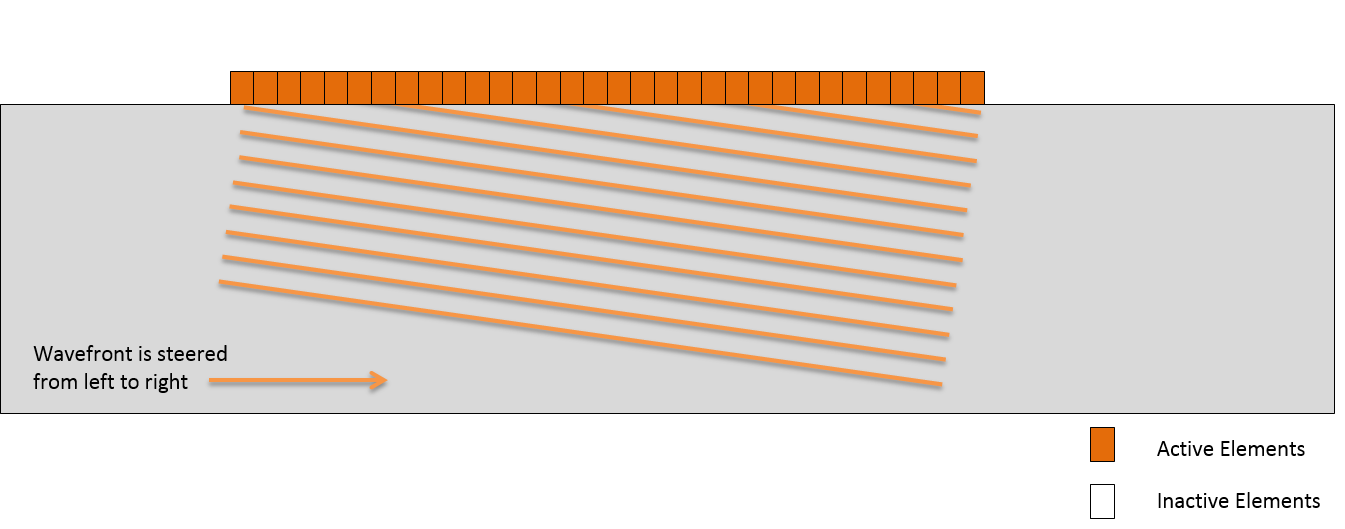
\includegraphics[width=\textwidth]{SectorB.png}
		\caption{An illustration of beam steering, used for the sector B-scan}
		\label{fig:SectorB}
\end{figure}

\subsubsection{Advanced Phased Array Imaging}\label{sec:advanced_pa_imaging}

The techniques described in the previous section are well established and have been used in ultrasonics for many years in both the NDE and medical fields. This subsection will introduce a number of advanced phased array signal processing methods that are designed to improve ultrasonic imaging via increasing both SNR and resolution.

The Phase Coherence Factor (PCF) is a technique that originated in medical imaging\cite{camacho_phase_2009} that has since been applied to NDE\cite{camacho_phase_2011}. The instantaneous phase of the signal can be calculated using the Hilbert transform. Using a standard delay-and-sum process, the standard deviation of phases at each point of focus is found. The standard deviation of the phases is used as an indicator of focal quality. For a well-focused beam, the standard deviation of the phases is very low. For an unfocused beam, the opposite is true. Using this knowledge, a weighting factor can be derived for the image so that the contributions from elements that are not well focused are minimised.

Minimum Variance beamforming, also known as Capon beamforming\cite{vignon_capon_2008}, applies an adaptive spatial filter to reshape the lobes of the signal\cite{sasso_medical_2005,asl_minimum_2009}. This technique has been well established in telecommunications and radar but has only comparatively recently been applied to ultrasonic imaging\cite{synnevag_minimum_2005}. The adaptive beamforming algorithm minimises the energy received from the medium while maintaining unity gain in a set direction. The minimum varience beamforming method was expanded upon through application of the Wiener beamformer\cite{nilsen_wiener_2010}. A range of adaptive weighting functions including Adaptive Sidelobe Reduction and Multiple Signal Classification (MUSIC) were investigated by DeGraaf\cite{degraaf_sidelobe_1994}. Computational complexity for these methods are a concern in the medical field\cite{nilsen_beamspace_2009} where real-time imaging is of utmost importance. Wang presented a minimum variance beamformer suited to high frame-rate imaging\cite{wang_mvdr-based_2009}, though he does not address computing power in his paper.

In delay-and-sum imaging, resolution can be improved through the minimisation of the main lobe width. This width affects the point spread function of an imaging system\cite{sakhaei_optimization_2006}. Jeong presented a method to scale received signals based on the ratio of main lobe to side lobe width\cite{jeong_fourier_2000}. Sakhaei investigated a similar frequency-domain technique in order to reduce sidelobe levels\cite{sakhaei_optimum_2012}.
A limitation of standard phased array processing techniques is that they are generally applied at the data acquisition stage and commercial phased array instrumentation often only outputs a processed signal. It is desirable to have the raw data so that data can be re-processed with modified parameters or entirely new algorithms.


\subsection{Full Matrix Capture}\label{sec:FMC}

In the previous section, delay-and-sum beamforming was introduced and reviewed and the methodologies for constructing an image evaluated. To provide a true focus for each pixel in an image, a transmission event would need to take place for each pixel. For a 500 by 500 pixel image, 250\e{3} transmissions are required. For a 1 kHz pulse repetition frequency (PRF), it would take 250 seconds to capture the relevant data to generate the image.

There is another methodology for collecting ultrasonic data from a medium. The Full Matrix Capture (FMC) process involves pulsing on a single element and recording the received signal at every element in the array. This is repeated, pulsing on each element of the array in turn. At the end of the process the time trace from every combination of transmit-receive pairs has been recorded\cite{holmes_post-processing_2005}. An illustration of the FMC acquisition procedure is shown in Figure \ref{fig:FMC1}. The data is stored in as a matrix of A-scans, $h$, and individual A-scans are referenced using the transmit-receive pair ($tx,rx$) they are associated with. An illustration of the matrix is shown in Figure \ref{fig:FMC2}. Individual samples of A-scans are referred to by their sample index, $(\psi)$.

\begin{figure}[htbp]
\centering
		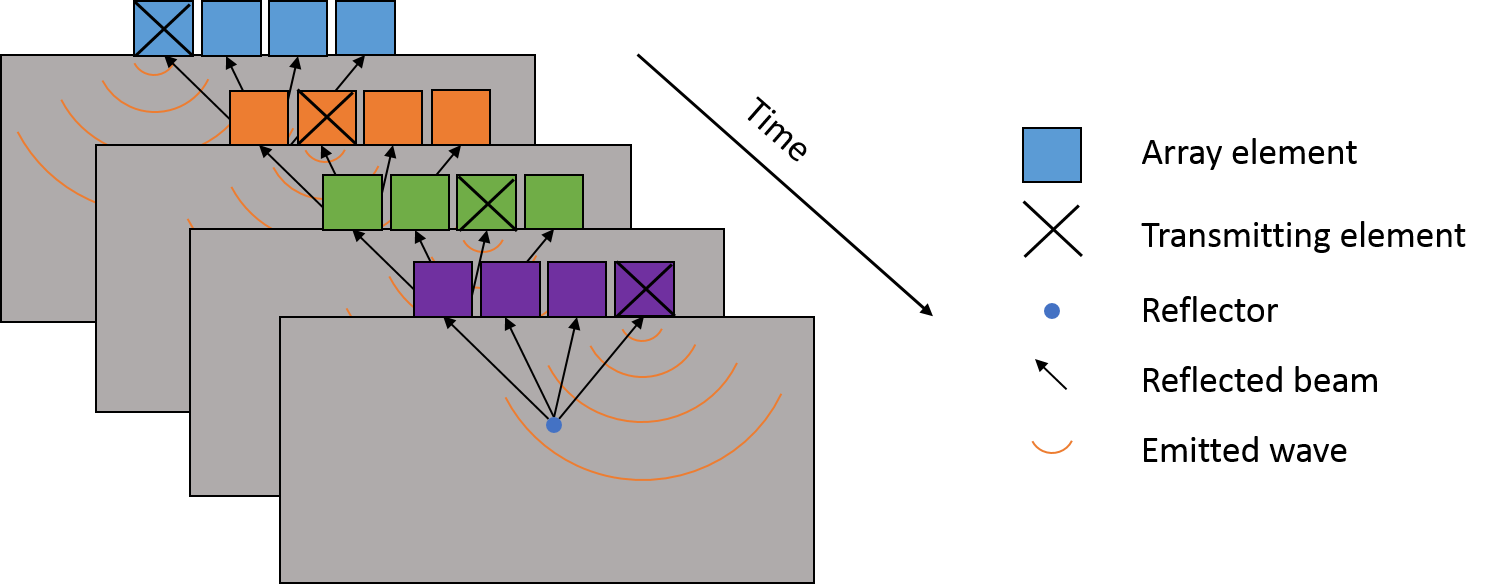
\includegraphics[width=\textwidth]{FMC.png}
		\caption{An graphic representation of Full Matrix Capture}
		\label{fig:FMC1}
\end{figure}

\begin{figure}[htbp]
\centering
		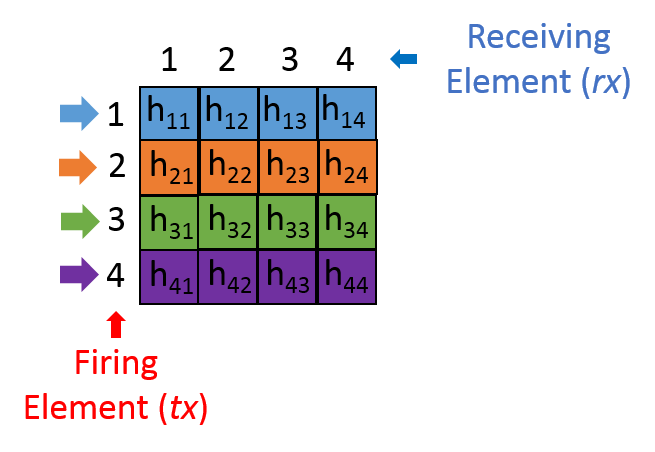
\includegraphics[width=80mm]{FMC_elements.png}
		\caption{An illustration of an FMC dataset}
		\label{fig:FMC2}
\end{figure}


Assuming that a medium has a linear response, and the principle of superposition holds true, the maximum amount of information able to be collected via an array has been recorded in the full matrix capture. Theoretically, any beamforming technique can be applied in post-processing with the Full Matrix Capture.

FMC is also more efficient when creating a high resolution image. For an array with 128 elements, assuming the same PRF as before, it would take 0.13 seconds (128 elements $\div$ 1kHz)  to record an FMC dataset. Any other limitations are a result of processing power, memory access speed and data transfer between instrument and PC.

\subsubsection{The Total Focusing Method}\label{sec:TFM}

One of the largest benefits of using FMC is that previously impractical imaging methods are now possible. The Total Focusing Method (TFM) is an example of this. It is an imaging algorithm that processes an FMC dataset in such a way that every pixel in an image is individually focused upon.

For every pair of transmitters and receivers, the round-trip propagation time is calculated to a specific pixel in a given image. This propagation time can be converted to an index for a sample ($\psi$) in an FMC dataset, given knowledge of the FMC's sampling rate and acquisition delay. The samples from each transmit-receive pair are summed and this process is repeated for every pixel in the image. The result is a TFM image. TFM images generally are superior in both SNR and resolution to focused or sector B-scan images. 

An example the TFM imaging process is shown in Figure \ref{fig:TFM_illus}. Every element is used to focus upon a single point and the response recorded for each element, as if there was a physically focused wavefront at that point. This is repeated for every pixel in the image to be generated.

The equation for calculating a 2D TFM image is shown in Equation \ref{eq:TFM}\cite{holmes_post-processing_2005}. 

 \begin{equation} \label{eq:TFM}
TFM(y,z) = | \sum h_{tx,rx} (\frac{\sqrt{(y_{tx} - y)^2 + z^2} + \sqrt{(y_{rx} - y)^2 + z^2}}{v_L}) |
 \end{equation}

\begin{figure}[htbp]
\centering
		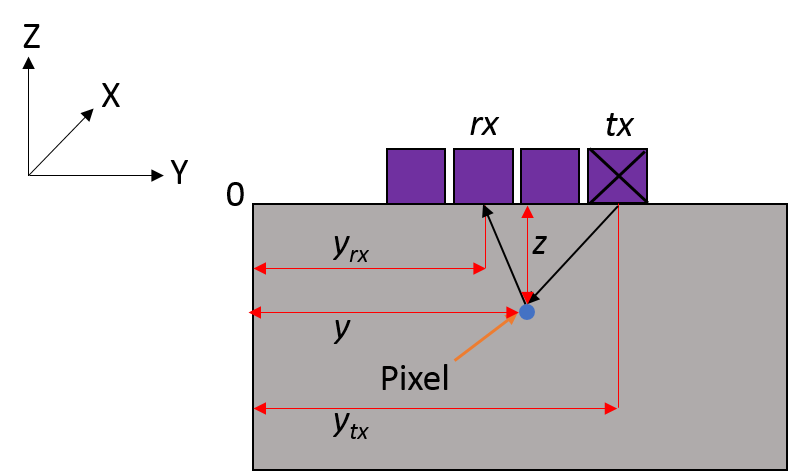
\includegraphics[width=80mm]{TFM2.png} \hspace{20mm}
		\caption{An graphical representation of the variables used in the TFM imaging process}
		\label{fig:TFM_illus}
\end{figure}

In Equation \ref{eq:TFM}, $y_{tx}$ and $y_{rx}$ are the x co-ordinates of the transmitting element and the receiving element of the probe, respectively. The $z$ co-ordinate of the probe are assumed to be zero i.e. that the image is centred around the interface of the probe and the load medium. $h_{tx,rx}$ represents the FMC data set and $v_L$ is the longitudinal velocity of propagation in the load medium. Finally, $y$ and $z$ represent the discrete location of the pixel to be processed. This is represented graphically in Figure \ref{fig:TFM_illus}.

Attention must be drawn to the orientation of the Cartesian plane which is depicted in Figure \ref{fig:TFM_illus} alongside the TFM scenario. This orientation is constant throughout this thesis and all reconstruction images are to be assumed to be in the 2D Y-Z plane unless otherwise stated.

TFM is a straight-forward technique which provides a synthetic focus at every discrete point in a given area (or volume) of the component under investigation. It does this by delaying the response from each array element to simulate a virtual focus at the point of interest. The contributions from each element are then summed and the TFM result is the signal magnitude at that point. The application of additional signal processing is common both before and after the reconstruction of the data. Filtering is often performed to remove electronic noise and any frequencies present in the signal that are outside the operational range of the array. After TFM imaging, a Hilbert transform can be applied to the resultant image in order to produce a smoother image\cite{ali_signal_2008}.

\subsubsection{Advanced Applications of the Full Matrix Capture}

The Vector Total Focusing Method (VTFM) allows additional information about the orientation of a crack to be gained\cite{wilcox_advanced_2007}.

The process is similar to TFM but for the contributions from each transmit element the amplitude and direction is recorded. These are summed as a vector and the resulting vector shows the direction of the source from where the most energy was reflected. This allows a greater understanding of reflector shape, orientation and type.

Camacho's Phase Coherence Imaging, introduced in Section \ref{sec:advanced_pa_imaging}, can be applied to FMC datasets. The principle remains the same, and in fact the process produces better results due to the fact that there are more samples contributing to a pixel, meaning there are more samples from which to calculate the standard deviation of phases.

Li and Li's Generalised Coherence Factor Imaging is similar to Phase Coherence Imaging\cite{li_adaptive_2003}. The Generalised Coherence Factor (GCF) calculates the ratio of energy in a defined area of the frequency spectrum to the energy in the full spectrum and uses this ratio to weight the TFM (or focused) image. For this method it assumes that the frequency profile of the coherent signals is known, and in fact it assumes it to be the low-frequency area of the spectrum. For materials that are difficult to inspect ultrasonically, this may not always be the case. This is a limitation of the GCF technique.

Gongzhang et al investigated methods of exploiting the larger range of frequencies recorded with wideband arrays. Frequency diversity techniques were used to remove speckle noise. This technique had the drawback of inserting a number of artefacts into both A-scans and images, affecting the probability of detection of genuine defects\cite{gongzhang_robust_2014,gongzhang_robust_2012}.

\section{Modelling Platforms}

Modelling is an important factor in designing arrays or post-processing methods. It allows multiple scenarios to be simulated both quickly and with less effort, compared to setting up experiments. The manufacture of numerous of arrays with differing configurations to test design parameters is not economically viable due to manufacturing time and costs.

\subsection{Finite Element}

The Finite Element method (FE) is a technique for simulating physical effects on models. Finite Element simulation is applicable in many areas of engineering due to its ability to solve complex problems and the fact that without it, many simulations would not be possible and experiments would have to be run every time data was required\cite{banerjee_elastic_2006}. The benefits of being able to gather information from a simulation as opposed to experimentally are numerous. The first is repeatability. Each time the experiment is run, the same data will be returned if the easily controllable parameters are kept the same. The second is ease of use; no complex phased array controllers need to be worked with, and a suitable sample does not have to be found. Parameters such as wave frequency can easily be changed and defects can be added to existing models.

The drawbacks to Finite Element modelling involve validity and time. There are many external factors when performing an ultrasonic inspection, including ambient temperature, thickness of couplant and array degradation. It is not practical to fully account for all potential factors and assumptions must be made. Because of this, results from experiment and modelling are rarely identical. The time taken to run large models can be an issue. Even fairly modest models can take hours to run with larger NDE models taking days, even on high performance computers. This pales in comparison to the field of geology where simulations may be run for many weeks to gather results.

Weidlinger Associates' PZFlex\cite{flex_web} was validated by Dobson et al to prove that the approximations that PZFlex makes will result in a valid model by comparing the results of a model to experimentally gathered data\cite{dobson_finite_2016}.


\subsection{Mathematical Modelling}

In Section \ref{sec:wave_eq} the wave equation was derived, with the following section dealing with the interaction of waves and boundaries. Section \ref{sec:huygens} introduced Huygens' principle of superposition and equations introduced which can be used to model the pressure field of an individual transducer of an array. The following section introduces mathematical modelling in the frequency domain, and a methodology for determining signal received by a transducer given an input signal and a knowledge of the system.

\subsubsection{The Frequency Domain}

The French mathematician, Fourier, demonstrated that frequency components in a linear system could be separated and analysed individually\cite{bracewell_fourier_2000}. Fourier's theorem states that any signal or image can be de-constructed and represented by a summation of a series of sinusoids\cite{szilard_ultrasonic_1982}.

The Fourier Transform is used to convert between the time and frequency domain analytically. The Fast Fourier Transform (FFT) is used in digital systems to perform an approximation of the Fourier Transform.

The Fourier Transform and its inverse can be expressed analytically as shown in Equations \ref{eq:review_freq_fft1} and \ref{eq:review_freq_fft2}.

\begin{equation} \label{eq:review_freq_fft1}
g(\omega) = F[f(t)] =  \int_{-\infty}^\infty f(t)e^{-i\omega t} dt
\end{equation}

\begin{equation} \label{eq:review_freq_fft2}
f(t) = F^{-1}[g(\omega)] = \frac{1}{2\pi} \int_{-\infty}^\infty g(\omega)e^{i\omega t} d\omega
\end{equation}

Any linear system can be represented as a transfer function and therefore the effects of propagation through a material can be considered as a transfer function applied to the input signal.

This transfer function can be represented as the product of individual effects of propagation. Figure \ref{fig:review_transfer} shows a graphical representations of the individual transfer functions, many of which are a function of frequency, that can be used to model wave propagation.

\begin{equation} \label{eq:review_freq_transfer}
H(\omega) = T_x(\omega) A(\omega) B_D X(\omega) \Delta(\omega) R_x(\omega)
\end{equation}

\begin{figure}[!ht]
\centering
		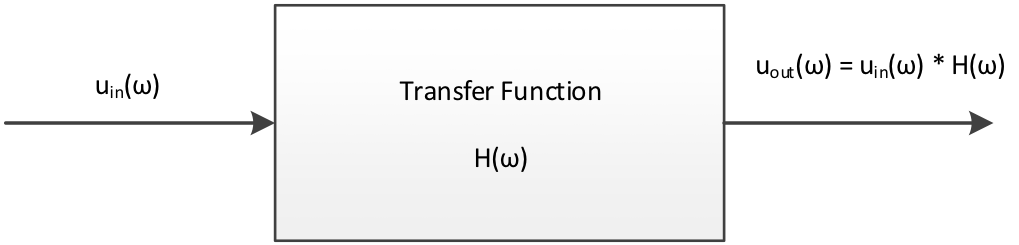
\includegraphics[width=10cm]{FreqSystem2.png}
		\caption{A graphical representation of a transfer function system}
		\label{fig:review_transfer}
\end{figure}

In Equation \ref{eq:review_freq_transfer}\cite{university_of_bristol_frequency_2011}, $T_x(\omega)$ represents the output of the transmitter; $R_x(\omega)$ is the characteristics of the receiver; $A(\omega)$ is the amplitude reduction due to attenuation; $B_D$ is the component representing the beam divergence; $X(\omega)$ represents the effects of boundaries encountered during propagation and $\Delta(\omega)$ is the time delay due to propagation. For a clean material with no features or reflectors, $X(\omega)$ may be set to $1$.

Both $T_x(\omega)$ and $R_x(\omega)$ are defined by the characteristics of the transmitter and receiver respectively. They are each the product of $I(\omega)$, which is the frequency response of the transducer, and $D_F(\omega)$, which is the angular sensitivity.

The characteristics of the transmitting and receiving transducers can be considered as the product of the respective frequency response and angular sensitivity (directivity) of each transducer.

The transfer function used to calculate propagation delay can be calculated as follows where $d$ is the propagation distance. It does not modify the amplitude of the signal, only the phase. $v_L$ can also be a function of $\omega$ as different frequencies may travel at different velocities. If this is the case, the signal will distort over distance. This is known as dispersion.

\begin{equation} \label{eq:review_freq_delay}
\Delta(\omega) = e^{\frac{-i\omega x}{v_L}}
\end{equation}

Attenuation rises exponentially with propagation distance and can be represented by Equation \ref{eq:review_freq_attenuation}, where is $\alpha$ the unit of attenuation, measured in Nepers per metre.

\begin{equation} \label{eq:review_freq_attenuation}
A(\omega) = e^{-\alpha x}
\end{equation}

The loss from beam spread (divergence) can be calculated simply, using Equation \ref{eq:review_freq_divergence}, where $x$ is the propagation distance.

\begin{equation} \label{eq:review_freq_divergence}
B_D = \frac{1}{\sqrt{x}}
\end{equation}

It is now possible to calculate the expected output at a receiving element using Equation \ref{eq:review_freq_transfer}, given that the transducer characteristics are known, the material properties of the medium that the signal will propagate through, and the input wave packet itself.

\subsubsection{Application of Mathematical Modelling}

A number of commercial software packages use mathematical modelling to calculate focal laws for inspection, such as UltraVision\cite{ultravision_web} (Zetec, USA) or CIVA\cite{civa_web} (CEA, France). More complex mathematical models have been achieved, simulating anisotropic materials in order to test image reconstruction methods\cite{humeida_simulation_2013}.

Dzieweirz and McGilp designed a process, using the mathematical modelling technique, to model an array and a point reflector in multiple locations to evaluate the performance of the array\cite{mcgilp_inspection_2014}. The mathematical modelling in this paper uses the same principles as the ones introduced in Section \ref{sec:wave_eq}. The Full Matrix Capture is simulated, the TFM image generated, and key metrics such as sensitivity and resolution are extracted. The data is compiled to a graph that shows the effective area of an array for a set of prerequisite metrics.

This process is computationally intensive, requiring thousands of separate simulation and imaging procedures. The process becomes more complex when coupling changes. When the array is not in contact with the medium to inspected, and water coupling is used, refraction will occur. A need arose to develop a rapid imaging platform which would take refraction into account and is the subject of the work developed in Chapter \ref{chap:cuetfm}.

% ------------------------------------------------------------------------


%%% Local Variables: 
%%% mode: latex
%%% TeX-master: "../thesis"
%%% End: 
